\documentclass[12pt, a4paper,oneside]{book}
% Подключение библиотеки
\usepackage{/Users/vladbelousov/Desktop/Semestr_4-FP-NSU/Настройка/library}
\usepackage{forest}

\begin{document}

\begin{titlepage}
    \thispagestyle{empty}  % Отключаем нумерацию страницы на титульном листе
    \centering
    \vspace*{1cm}  % Отступ сверху

    \textbf{\huge Конспект лекций по дисциплине}  \\[1.5cm]  % Название
    \textbf{\huge Основы функционального анализа}  \\[2cm]   % Название дисциплины (оставьте пустым для добавления вручную)
    \textbf{\Large Новосибирский государственный университет} \\[0.5cm]
    \textbf{\large Физический факультет} \\[0.5cm]
    \textbf{\large 4-й семестр} \\[0.5cm]
    \textbf{\large 2025 год} \\[10cm]

    \begin{flushright}
        \large Студент: Б.В.О \\[0.5cm]  % Ваше имя
        Преподаватель: Ротанова Татьяна Александровна  % Ф.И.О. преподавателя
    \end{flushright}
\end{titlepage}

\tableofcontents  % Создание оглавления

\def\mainfile{}  % Определяем макрос для основного файла
%Февраль
% Условная компиляция для самостоятельной работы
\ifdefined\mainfile
    % Если это часть основного файла, не добавляем начало и конец документа
\else
    \documentclass[12pt, a4paper]{report}
    \usepackage{/Users/vladbelousov/Desktop/Semestr_4-FP-NSU/Настройка/library}
    \usepackage[utf8]{inputenc} % Подключение поддержки UTF-8
    \begin{document}
\fi

%%-------------------------------%%

\chapter{Геометрия пространств со скалярным произведением.}

\begin{center}
    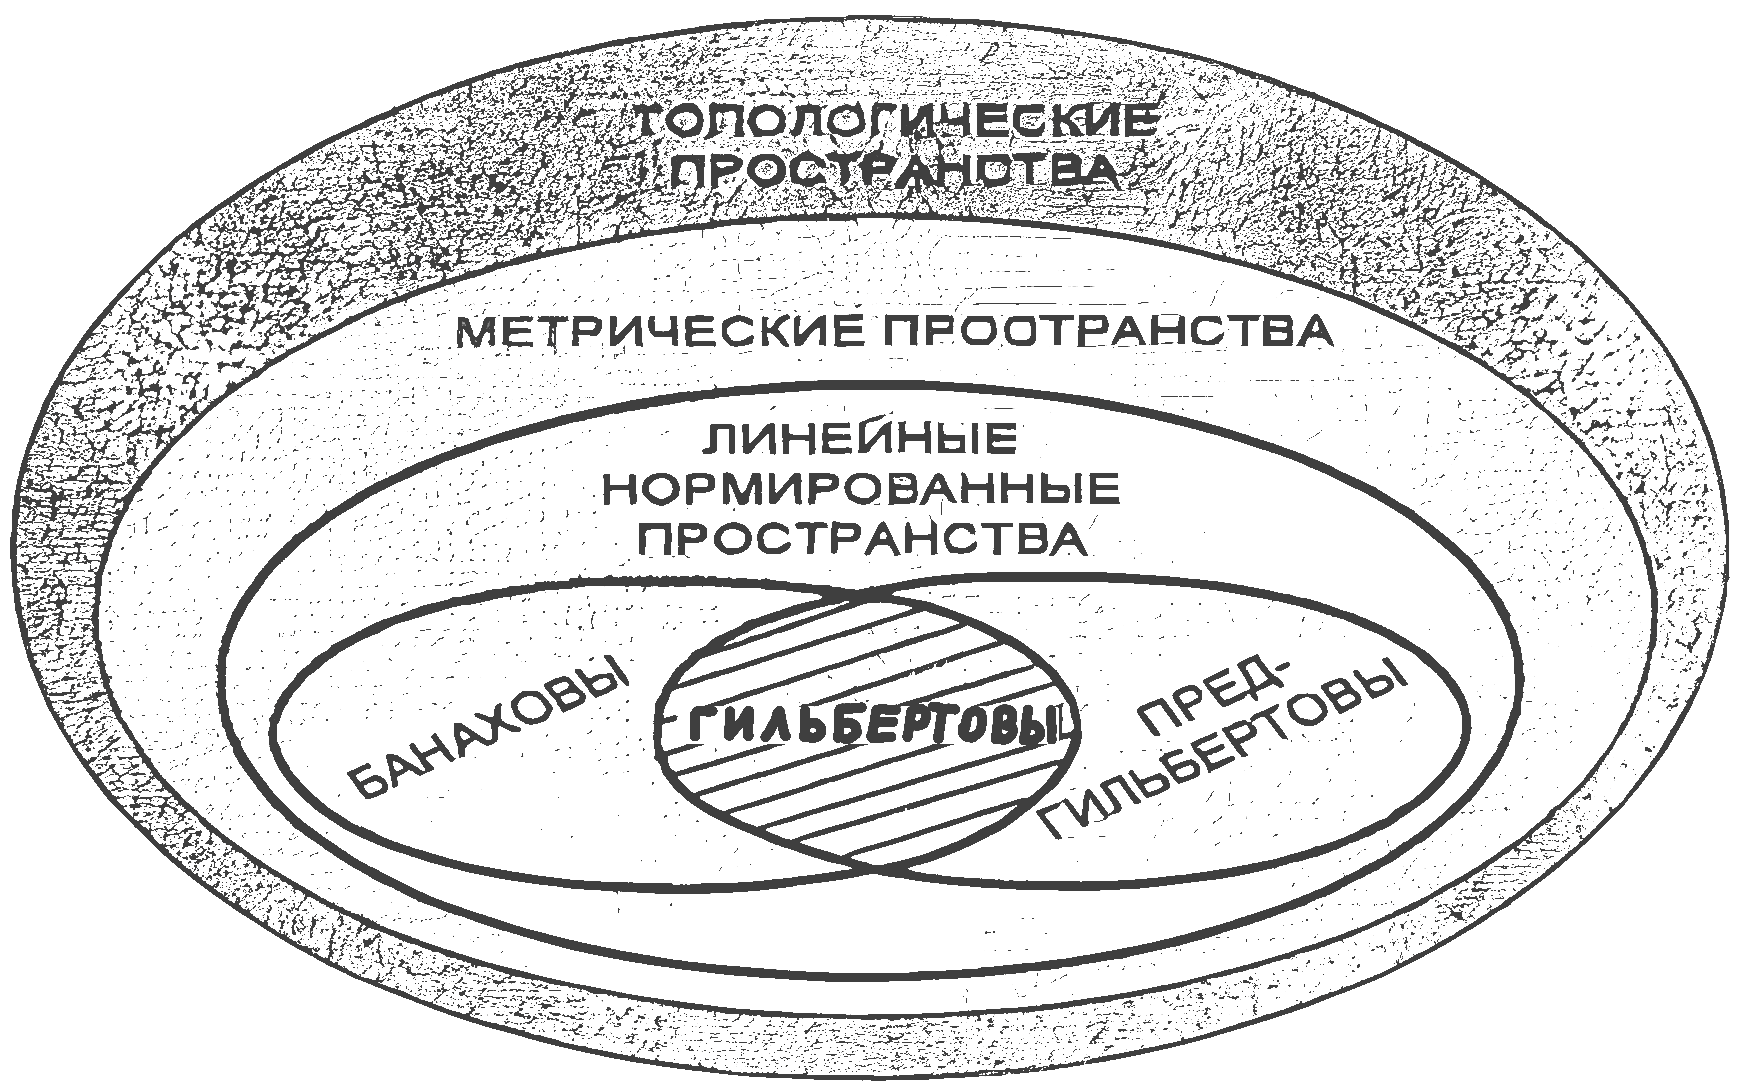
\includegraphics[width=0.5\textwidth]{/Users/vladbelousov/Desktop/Semestr_4-FP-NSU/ОФА/Лекции_по_дням/image/1.png}
\end{center}

\begin{definition}[Метрическое прострнвство]
    Метрика \( \rho (x,y): M ^2 \to  \mathbb{R} \) 

    1) \( \forall x,y :\rho (x,y ) \geq 0 - ( \rho(x,y) = 0 \Leftrightarrow x=y)   \) 

    2) \( \forall x,y \in  M :\rho(x,y )= \rho (y,x)  \)
    
    3) \( \forall x,y,z :\rho(x,z) \le  \rho(x,y)+\rho(y,z) \)
\end{definition}

\( B_{\varepsilon}(x) = \{ y \in  M | \rho(x,y) < \varepsilon \} \) 

\begin{definition}
    Множество открытое, если любая точка в нем содержится в нем вместе некоторой окрестностью.
\end{definition}

Пример дискреткой метрики: 

\[ 
\rho(x,y) = 
\begin{cases} 
    1 \quad x \neq y \\
    0 \quad  x=y   
\end{cases} 
\] 

\section{Линейно (векторное) пространство}

\begin{definition}
    Непустое множество элементов L произвольной природы, называется линейным (векторным) над полем чисел \( \mathbb{R} (\mathbb{C})\) если 

    1) \( \forall x,y   \) введена операция сложения:

    \( \quad  \) 1.1)  \( x+y = y+x \) (коммутативность)
    
    \( \quad  \) 1.2) \( x+(y+z)= (x+y ) +z \) (ассоциативность)
    
    \( \quad  \) 1.3) В L существует элемент называемым нулем 0: \( x+0 = x \text{ }  , \forall x \in  L \)  

    \( \quad  \) 1.4) \( \forall x \in  L \)  существует противоположный элемент принадлежащий 
    
    L: \( x+y = 0 \) , обозначается как \( -x \)

    2) \( \forall x \in  L \)  и \( \forall  \) числа \( \alpha \in  \mathbb{R}(\mathbb{C}) \) определен вектор из L - произведения элементов на число \( \alpha , \alpha x \in  L \):
    
    \( \quad  \) 1.1) \( \alpha (\beta x )= (\alpha \beta )x  , \forall  \alpha, \beta  \)
    
    \( \quad  \) 1.2) \( 1 \cdot x =x  \) (существования единицы)
    
    \( \quad  \) 1.3) \( \alpha (x+y) = \alpha x + \alpha y \)

    \( \quad  \) 1.4) \( (\alpha + \beta )x = \alpha x + \beta x \) 


\end{definition}

Примеры: 

1)
\[ \begin{aligned}
\begin{array}{ll}
    \mathbb{R}^{n }\\
    \mathbb{C}^{n}  
\end{array}
\begin{array}{ll}
    \quad \alpha(x_1,x_2, \ldots, x_n) \\
    + \\
    \quad \beta (y_1,y_2, \ldots ,y_n )
\end{array}
\quad =(\alpha x_1 + \beta y_1 ,\dots \alpha x_n + \beta y_n)
\end{aligned} \] 

2) \( C[a,b] = \{f(a,b) \to  \mathbb{C}, \text{ непрерывная функции } f \text{ - непрерывна }   \)\}

3) \(\displaystyle  L_p (x)= \{f \text{- измерима по Лебегу, заданная на } X , f: X \to  \mathbb{C} \text{ таких, что }   \)

\[  \int_{X}|f(x)|dx< \infty  \] 

4) \(\displaystyle  l_2 : x = \{x_1 , \ldots , x_n  \} \quad \sum ^{\infty }_{1}  |x_n| ^2 < \infty  \) 

\begin{definition}
    \( x_1, \ldots, x_n \)  называется линейно зависимыми, если \( \exists \alpha_1 , \ldots , \alpha _ n   \) не все равные нулю, такие что \( \alpha_1 x_1 + \dots + \alpha_n x_n=0   \)
    
    В противном случае: из того, что \( \alpha_1 x_1 + \dots + \alpha_n x_n=0 \) следует, что все \( \alpha_i =0  \) \( x_1, \ldots, x_n \)  называется линейно независимыми наборами  векторов.  
\end{definition}

\begin{definition}
    Бесконечный набор элементов L называется линейно независимым, если любой его конечный поднабор линейно независимым.
\end{definition}

\begin{definition}
    Если в L можно найти \( n  \)  линейно независимых векторов, а любой набор из \( n+1 \) векторов является линейно зависимыми, то \( \dim L= n \). Если в L можно указать   набор из произвольного числа линейно независимых элементов, то \( \dim L= \infty  \). 
\end{definition}

\begin{definition}
    Непустое подмножество \( S \subset L  \)  называется подпространством, если оно само является пространством введенных в L линейных операций.
\end{definition}

\begin{definition}
    Линейной  оболочкой  <M> называется совокупность всех линейных комбинаций  \( \alpha x + \beta y  \)  где \(  x,y \in  M  \subset \alpha, \beta \in  \mathbb{C}(\mathbb{R}) \) 

    <M> - подпространство в L  (натянутое или порожденное множеством элементов M)
\end{definition}


\begin{definition}
    Норма в линейном пространстве L:  \( \norm{\text{ } }  : L \to  \mathbb{R}^+ = [ 0 , \infty ) \)

    \( \forall x,y \in  L ,  \forall  \alpha \in  \mathbb{C}(\mathbb{R}) \) 
    
    1) \( ||x|| \geq  0 ,||x||=0 \Leftrightarrow x=0  \quad   \) (положительная определенность нормы)
    
    2) \( ||\alpha x||=|\alpha|||x || \quad  \)  (положительная однородность нормы) 

    3) \( ||x+y|| \le  ||x|+||y|| \)
\end{definition}

В конечномерных пространствах все нормы эквиваленты \( c_1||x||_1 \le  ||x||_2 \le  c_2 ||x||_1 \). В конечномерных пространствах это не так! 

Пример норм: 

\[1)  \norm{f}= \max _{t \in [ a,b]} |f(t)| \text{ - норма в }  C [ a,b]  \text{ равномерная норма.}  \] 

\[ \begin{aligned}
    2) &  \quad ||f||_{L_1} = \int_{X} |f|dx \text{ в  }  L_1 \\
    3) & \quad ||f||_{L_p} = \sqrt[p]{\int_{X}|f|^p dx} \text{в}  L_{p} \\
    4) & \quad ||x||_{l_2}= \sqrt{\sum^{\infty }_{i=1} |x_i| ^2   }   
\end{aligned} \] 

\begin{definition}
    Последовательность \( (x_n)_{n \in  N}  \) точек линейно нормированное пространств L сходятся к x, если  \( ||x_n - x|| \xrightarrow{n \to  \infty } 0 ,\forall \varepsilon > 0, \exists n_0, n > n_0 : ||x_n - x|| < \varepsilon   \) 
\end{definition}

\begin{definition}
    Предельной точкой \( M \subset L  \)  называется точка x, если существует сходящаяся к x последовательность элементов из M \( \exists x_n \in  M : x_n \to x  \) 
\end{definition}

\begin{definition}
    Замыканием \( \overline{M}  \) - объединение  M и его предельных точек (по конкретной норме). 
\end{definition}

\begin{definition}
    Множество замкнутое, если содержит все предельные точки.
\end{definition}

\begin{definition}
    Множество M в L - линейно нормированном пространстве называется плотным в L, если \( \overline{M}= L  \) 
\end{definition}

\begin{definition}
    Сепарабельное множество, если в нем \( \exists  \) счетное плотное подмножество
\end{definition}



%%-------------------------------%%

% Закрытие документа, если файл компилируется отдельно
\ifdefined\mainfile
    % Если это основной файл, не нужно заканчивать документ
\else
    \end{document}
\fi
% Условная компиляция для самостоятельной работы
\ifdefined\mainfile
    % Если это часть основного файла, не добавляем начало и конец документа
\else
    \documentclass[12pt, a4paper]{report}
    \usepackage{/Users/vladbelousov/Desktop/Semestr_4-FP-NSU/Настройка/library}
    \usepackage[utf8]{inputenc} % Подключение поддержки UTF-8
    \begin{document}
\fi

%%-------------------------------%%

Пример: Множество множеств P[0,1] не является замкнутым подпространством в C[0,1]

\[ P_n (x )  \to  f(x ) \Leftrightarrow  \left\lVert P_n - f  \right\rVert _C \to  0 \]

\[ \forall  n , p_n \in  P[0,1] , f(x ) \in  C[0,1] - \text{не является полиномом} \] 

\[ p_n(x) = 1+ x + \frac{x ^2 }{2 }  + \dots + \frac{x^n }{n!}  \] 

\[  f(x ) = e ^{x} , \quad f(x ) = f(0 ) +\frac{f'(0)}{1!}x+\frac{f''(0 )}{2!}x^2+\dots+ \frac{f^{(n )(0)} }{n ! }x^{n } + \frac{f^{(n+1 )(c)} }{(n+1)!} x^{n+1}     \] 

Замыкание \( P[0,1] \)  это \( L_2[0,1] \) 

\[ \left\lVert p_n -f  \right\rVert _{L_2}  \le  \max_{x \in [0,1]} \max_{c \in  [0,1]} \left\lvert \frac{e^c x^{n+1 } }{(n+1)!}  \right\rvert  \overset{\tiny\begin{aligned} x=1 \\c=1\end{aligned}}{=}\frac{e}{(n+1)!} \xrightarrow{n \to  \infty } 0 ,\quad e^x \notin P[0,1]       \] 



\[ L_2 (x ) :\{f: X \to  Y , \int_{x} |f| ^2 dx < \infty \} \] 

\[ \left\lVert f  \right\rVert _{L_2 } = \sqrt{\int_{x }|f| ^2 dx} \] 

Нуль: \( f : X \to  Y  \) 

\[  0(x ) : X \to  Y \] 

\[ g=0(x ) = 0 - \text{почти всюду}  \] 

\[ g = \begin{cases}
    0 , \mathbb{R}  /\mathbb{Q} \\
    \infty , \mathbb{Q}  
\end{cases} \] 


Элементы (вектора) пространства \( L_2    \)  - функции класса \( L_2  \) .

\begin{definition}
    Последовательность \( (x_n )_{n \in  \mathbb{N}} , x_n \in  L \) (линейно нормированное пространство) называется фундаментальной, если \( \forall  \varepsilon >0 , \exists N , \forall m,n >N : \left\lVert x_m - x_n  \right\rVert < \varepsilon \) 
\end{definition}

\begin{definition}
    Если любая фундаментальная последовательность является сходящейся в L, то L - полное пространство.
\end{definition}

\begin{definition}
    Полное нормированное пространство - банахово пространство
\end{definition}

\section{Линейные пространства с скалярным произведением}

\begin{definition}
    Скалярное произведение в L (, ) : \( L \times L \to  \mathbb{C} \). \( \forall x_1,x_2, y \in  L, \alpha_1,\alpha_2 \in \mathbb{C}(\mathbb{R}) \) выполняется: 

    1) \( (\alpha_1 x_1 + \alpha_2 x_2, y ) = \alpha_1(x_1,y )+ \alpha_2 (x_2,y) \) 

    2) \( (x,y ) = (\overline{y,x} )\)  

    3) \( (x,x ) \ge  0 \quad \text{и}  \quad  (x,x ) = 0 \Leftrightarrow x =0\) 
\end{definition}

Линейное пространство со скалярным произведением над \( \mathbb{R}   \) - евклидовы пространства, над \( \mathbb{C}    \) - унитарное пространства. 

\[ 1) \mathbb{R} ^ n ( \mathbb{C}^ n ): (x, y ) = \sum  ^{n }  x_i \overline{y } _i   \] 

\[ 2) l_2 : (x,y ) = \sum ^{\infty  } x_i \overline{y } _i   \] 

\[ 3) L_2(x ) : (f,g )= \int  _{x } f \overline{g } dx   \] 

\[ 4) C[a,b ] : \text{ нет скалярного произведения согласованного  с аксиомами нормы} \] 

\begin{lemma}
    Величина \( \left\lVert x  \right\rVert = \sqrt{(x,x)} \) удовлетворяет свойствам нормы. Согласованная или порожденная скалярным произведением.
\end{lemma}


\begin{definition}
    Гильбертово пространство - пространство со скалярным произведением, полное относительно нормы, порожденным этим скалярным произведением.
\end{definition}

\begin{lemma}[ Неравенство Коши-Буняковского]
    \( \forall x \in  L \quad  |(x, y )| \le  \left\lVert x  \right\rVert \left\lVert y \right\rVert \) 
\end{lemma}

\begin{proof}
    \[ \alpha = \frac{(x,y )}{|(x,y )|} , \quad  t \in  \mathbb{R} \] 

    \[ 0 \le  \left\lVert \overline{\alpha} x +  ty \right\rVert ^2 = ( \overline{\alpha } x+ ty , \overline{\alpha } x + ty     ) = \overline{\alpha }( x, \overline{\alpha }x _ty  ) + t(y , \overline{\alpha }x + ty  )=   \] 

    \[  \underbrace{|\alpha | ^2}_{=1} ( x,x ) + \overline{\alpha } t ( x,y ) + \alpha t ( y ,x ) + t ^2 ( y,y )=  \left\lVert x  \right\rVert ^2 + \overline{\alpha } t (x, y ) + \alpha t ( y ,x ) + t ^2 \left\lVert  y  \right\rVert ^2 \boxed{=}    \] 

    \[\overline{\alpha }t (x,y )+ \alpha t ( y ,x )  =t  \left( \frac{(\overline{x,y }  ) ( x,y)}{|(x,y)|}+ \frac{({x,y }  ) (x,y)}{|(x,y)|} \right)  = 2t |(x,y)|\] 

    \[ \boxed{=} \left\lVert x   \right\rVert  ^2 + 2t |(x,y)   |+ t ^2 \left\lVert y  \right\rVert ^2\] 

    \[ |(x, y )| \le  \left\lVert x  \right\rVert \left\lVert y \right\rVert \] 
\end{proof}

\begin{proof} [Доказательство Леммы 1]

    1) Из 3 аксиомы скалярного произведения; 

    2) \( \alpha \in  \mathbb{C}, \left\lVert \alpha x    \right\rVert ^2 = |\alpha | ^2 \left\lVert x  \right\rVert ^2 =(1) \)
    
    \[ (\alpha x , \alpha x ) = \alpha ( x, \alpha x ) = \alpha \overline{\alpha } ( x,x)  = (1 ) \] 

    3) \( \left\lVert x + y  \right\rVert \le  \left\lVert x  \right\rVert \left\lVert y \right\rVert \) 

    \[ \left\lVert  x+ y  \right\rVert ^2 = ( x+ y , x+ y )  = ( x, x+ y ) + ( y , x+ y ) = ( \overline{x+ y , x }  ) + ( \overline{x+ y , y }  ) = (\overline{x,x }   ) + ( \overline{y,x }   )  +( \overline{x, y }  ) + ( \overline{y, y }  ) = \] 

    \[ = \left\lVert  x  \right\rVert  ^2 +  (x, y ) + (y,x ) +  \left\lVert y  \right\rVert ^2 \le  \left\lVert x  \right\rVert ^2 + 2 |(x,y)   | + \left\lVert y  \right\rVert ^2  \le  \] 

    \[ \overset{\text{нер-во К-Б} }{\le}  \left\lVert x  \right\rVert ^2 + 2 \left\lVert x  \right\rVert \left\lVert y  \right\rVert+ \left\lVert y  \right\rVert ^2 = ( \left\lVert  x  \right\rVert + \left\lVert  y  \right\rVert) ^2  \] 
\end{proof}


\[ L_2 : \sqrt{ \int  _x |f(x)| ^2 dx    } = \left\lVert f  \right\rVert _{L_2}  \] 

\[ \left\lvert \int_{x }  f (x ) \overline{g }  (x ) dx        \right\rvert  \le  \left( \int_{x }|f(x ) | ^2 \right) ^{\frac{1}{2 } } \left( \int_{x } |g(x)| ^2 dx   \right) ^{\frac{1}{2} } - \text{ неравенство К-Б в }  L_2     \] 

\[ \sqrt[  p ]{\int_{x }|f(p)|dx}= \left\lVert f  \right\rVert _{L_p} \]  

\begin{lemma}
    \( \forall p \geq 1   \) линейно нормированное пространство  \( L_ p   \)  является полным.  
\end{lemma}

\begin{lemma}
    \( \forall  p \geq 1   \)  пространство \( C^{\infty }  \) плотно в \( L_p (x) \), то есть \( \overline{C}^{\infty ^{L_p} }= L_p(x)    \)   
\end{lemma}

\begin{lemma}
    \( \forall  p \ge 1  \)  пространство \( L _ p  \)  сепарабельно.
\end{lemma}

\begin{lemma}
    Пусть L - линейно нормированное пространство со скалярным произведением и норма порождена скалярным произведением\dots

    \[ \forall  x, y \in  L \quad  \left\lVert x+ y  \right\rVert ^2 + \left\lVert  x- y  \right\rVert ^2 = 2 (\left\lVert x   \right\rVert ^2 + \left\lVert y  \right\rVert ^2) - \text{равенство паралеллограма} \] 
\end{lemma}

Наоборот, если в линейно нормированном пространстве L выполняется равенство паралеллограма, то в этом пространстве можно ввести скалярное произведение, согласованной с этой нормой.

\( L_1 \subset [ a, b ] \exists  f,g ,   \)  для которых не выполняется равенство паралеллограма \( \Rightarrow      \) нельзя ввести скалярное произведение, согласованное с нормой.

\begin{lemma}
    В линейном  пространстве со скалярным произведением  L , скалярное произведение непрерывно по первому аргументу относительно сходимости по норме порожденной скалярным произведением

    \[ x_n \to  t \quad \left\lVert x_n - x           \right\rVert  \xrightarrow{n \to  \infty }  0  \] 

    \[ \forall y , (x_n, y  ) \to  (x, y ) \] 
\end{lemma}

\begin{proof}

    \[ |(x_n, y ) -(x,y )  | = |(x_n- x,y ) | \overset{\text{по К.Б} }{\le}  \left\lVert x_n - x  \right\rVert \underbrace{\left\lVert y \right\rVert}_{\text{огр.числено} } \xrightarrow{x \to  \infty } 0   \] 
\end{proof}

\section{Ортогональность векторов}

\begin{definition}
    L  - пространство со скалярным произведением, \( x, y \in  L \) называется ортогональным, если \( (x,y ) = 0   \) 

    
\end{definition}

\begin{definition}
    Набор векторов \( x, \ldots, x_n, \ldots,   \in  L \) называется ортогональным, если \( \forall  ij : x_i \perp x_j  \) 
\end{definition}


\begin{definition}
    Набор ортогональный ( \( x_n     \) ) называется ортнармированным, если \( \forall  i :  \left\lVert x  \right\rVert = 1   \) 
\end{definition}

Ортогонализация Грамма-Шмидта

Если \( x_1, \ldots, x_n  \)  - счетная система линейно назависимый в  L , тогда новые последовательности: 

\[ y_1 = x_1 \quad  z_1 = \frac{y_1}{\left\lVert y_1  \right\rVert}  \] 

\[ y_2 = x_2 - ( x_2 , z_1 ) z_1  \quad  z_2 = \frac{y_2}{\left\lVert y_2  \right\rVert} \] 

\[ y_n = x_n - \sum ^{n-1 }_{k =1}( x_n , z_k ) z_k  \quad  z_n = \frac{y_n}{\left\lVert y_n  \right\rVert}    \] 

Обладает свойствами: 

1) Система \( z_1, \ldots, z_n   \) - ортонормированна

2) \( \forall n \in  N \underset{\text{линейные оболочки } }{\underbrace{<z_1, \ldots, z_n >} = \underbrace{<x_1, \ldots, x_n>}}\) 
%%-------------------------------%%

% Закрытие документа, если файл компилируется отдельно
\ifdefined\mainfile
    % Если это основной файл, не нужно заканчивать документ
\else
    \end{document}
\fi
% Условная компиляция для самостоятельной работы
\ifdefined\mainfile
% Если это часть основного файла, не добавляем начало и конец документа
\else
\documentclass[12pt, a4paper]{report}
\usepackage{/Users/vladbelousov/Desktop/Semestr_4-FP-NSU/Настройка/library}
\usepackage[utf8]{inputenc} % Подключение поддержки UTF-8
\begin{document}
\fi

%%-------------------------------%%

\begin{definition}
     Углом между ненулевыми векторами x и y  евклидова пространства \( L  \)  называется число \( \varphi \in  [ 0, \pi ] \):

     \[ \cos \varphi = \frac{(x,y )}{\left\lVert x  \right\rVert \left\lVert y  \right\rVert}  \] 
\end{definition}

\begin{definition}
    Если S - подпространство пространства со скалярным произведением \( L \), то \( x \in  S  \)  называется вектором наилучшего приближения (ближайший) для \( y \in L      \)  посредством векторов из \( S  \), если: 

    \begin{center}
        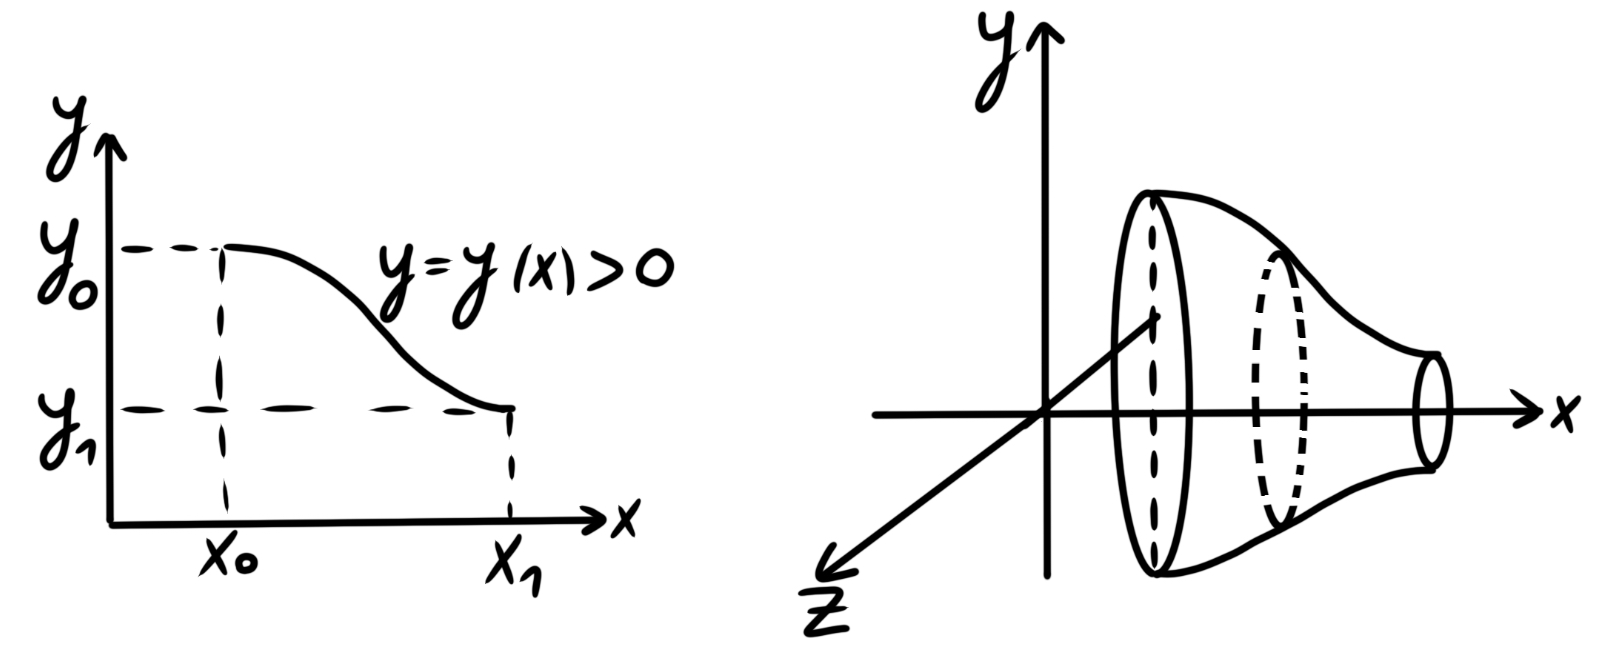
\includegraphics[width=0.3\textwidth]{/Users/vladbelousov/Desktop/Semestr_4-FP-NSU/ОФА/Лекции_по_дням/image/2.png}
    \end{center}

    \[ \forall z \in  S , \quad  \left\lVert y - z  \right\rVert \geq  \left\lVert x - y  \right\rVert \] 

    \[ \left\lVert x - y  \right\rVert  = \inf _{z \in  S } \left\lVert y -z  \right\rVert  \] 
\end{definition}

\begin{theorem}
    Пусть \( H  \)   - гильбертово пространство, \( S  \)   - замкнутое подпространство \( H , \text{  }  y \in  H  \), тогда \( \exists  ! x  \) ближайший к y.
\end{theorem}

\begin{proof}

    \[ \inf \left\lVert y -z  \right\rVert = d  \]  

    \[ x_1, \ldots, x_m \in  S \quad  \left\lVert  y - x_m       \right\rVert \xrightarrow{m \to  \infty } d   \] 

    \[ \left\lVert x_m - x_n         \right\rVert ^2 = \left\lVert (x_m - y ) - (x_n - y )  \right\rVert  ^2 = 2( \left\lVert  x_m - y   \right\rVert ^2 + \left\lVert  x_n - y      \right\rVert ^2 ) - \underset{_{\left\lVert x_m+ x_n - 2y  \right\rVert ^2 = 4 \left\lVert q - y  \right\rVert ^2 \geq 4 d ^2  }}{\left\lVert \underbrace{x_m - y + x_n - y }  \right\rVert }^2 \boxed{\le } \] 

    \[ q = \frac{x_m+ x_n }{2 } \in  S   \] 

    \[  \forall  \varepsilon , \exists  N \text{ }  n, m \geq  N :  \left\lVert x_m - y      \right\rVert  < d ^2 + \varepsilon \quad  \left\lVert  x_n - y  \right\rVert  ^2 \le  d ^2 + \varepsilon \] 

    \[ \boxed{\le  } 4 d ^2 + 2 \varepsilon - 4 d ^2 = 2 \varepsilon   \] 

    \[ x_m - \text{ фундаментальная }  \] 

    \[ \text{существование предела последовательности }   x: \] 

    \[  x \in  S , \text{ т.к }  S - \text{ замкнутое}  \] 

    \[ \left\lVert  y - x_n      \right\rVert = \sqrt{(y - x_n , y - x_n )} \underset{(1)}{\xrightarrow{n \to  \infty  } }\sqrt{(y - x, y -x )} = \left\lVert y -x  \right\rVert \to  d \text{ в силу ! предела}    \] 

    \begin{center}
        (1) - непрерывность по 1-му аргументу
    \end{center}

    Единственность: 

    \[ \text{Пусть } \tilde{x }: \left\lVert  y - \tilde{ x }\right\rVert = d , x \neq  \tilde{x } \] 

    \[ \left\lVert  \tilde{ x } - x      \right\rVert ^2 = \left\lVert  (\tilde{x }- y ) - ( x - y ) \right\rVert ^2 = 2\underset{= d ^2 }{\left\lVert \underbrace{\tilde{x }  - y}  \right\rVert}  ^2 +2\underset{= d ^2 }{\left\lVert \underbrace{x  - y}  \right\rVert} ^2 - \left\lVert 2 y - x - \tilde{x } \right\rVert ^2 \le 4 d ^2 - 4 d ^2 \le  0 \] 

    \[ \text{т.е } \tilde{x } = x - \text{ противоречие }  \] 

\end{proof}

\begin{definition}
    \( S  \)  - подпространство в линейном пространстве со скалярным произведением \( L, \text{ } x \in  S   \)  - ортогональная проекция \(  y \in  L   \)  на подпространство \( S  \), если: 

    \[ y- x \perp  S \quad  y -x \perp  z \text{ }  \forall  z \in  S \quad  ( y - x , z ) = 0  \] 

\end{definition}


\begin{lemma}
    \( S  \)  - подпространство в линейном пространстве со скалярным произведением \( L, \text{ }  x \in  S  \)  - ортогональная проекция \(  y \in  L  \Leftrightarrow   \)   x - ближайший к y посредством S.
\end{lemma}

\begin{proof}

    \[  \] 

    \( \boxed{\Rightarrow} :\) 
    
    \[ \forall  x, y , z \in  L \] 

    \[ \left\lVert  y - z  \right\rVert ^2  = ((y -x )+ (x- z ), (y -x) + ( x - z)) =   \] 
    
    \[ \overset{(1)}{=} \left\lVert y -x    \right\rVert ^2 + 2 \mathrm{Re }( \cancelto{0 }{x- y , x -z }) + \left\lVert x -z  \right\rVert ^2 (* ) \] 

    \[ (1): (a+b, a+ b )   = \left\lVert  a  \right\rVert ^2 + \left\lVert  b  \right\rVert ^2 + 2 \mathrm{Re } ( a,b ) \] 

    \[ x \in  S - \text{ ортогональная проекция y  на }  S \Rightarrow y -x \perp  x-z   \]  

    Итого: 

    \[ \left\lVert  y -z  \right\rVert ^2 = \left\lVert  y -x  \right\rVert ^2 + \underset{\geq 0 }{\left\lVert \underbrace{ x- z}  \right\rVert }^2  \] 

    \[ \forall  z \in  S : \left\lVert  y -z  \right\rVert ^2 \le  \left\lVert  y -x  \right\rVert ^2 , x - \text{ ближе для y }  \] 

    Пусть дано: 

    \( \boxed{\Leftarrow}: \) 

    \[ x - \text{ ближайший вектор для  } y \in S   \] 





    \[ \begin{aligned}
        \begin{array}{l|}
            \left\lvert y -x  \right\rvert = \inf \left\lVert  y -z \right\rVert \\
            f(t )  = \left\lVert  y -x + t W  \right\rVert ^2, \quad  t \in  \mathbb{R}  ^2 , \text{ }  W \in S
        \end{array}
        \Rightarrow f' (0 ) =0 
    \end{aligned} \] 

    \[ \lim_{t  \to 0}  \frac{ \left\lVert y -x + t W  \right\rVert ^2 - \left\lVert  y -x  \right\rVert ^2 } {t } = 0   \] 

    \[ \text{ в } (* ): z = x - t W  \]
    
    \[ \left\lVert y - (x - tW ) \right\rVert  ^2 - \left\lvert y -x  \right\rvert  ^2 = 2 \mathrm{Re } (y - x, t W ) + \left\lVert t W  \right\rVert ^2   \] 

    \[ \lim_{t  \to 0}    t\frac{2 \mathrm{Re } (y - x , W ) }{ t } + t ^2         \cancelto{0 }{ \frac{\left\lVert W  \right\rVert ^2 }{t } } = 0      \] 

    \[ 2 \mathrm{Re }  ( y - x, W )  = 0  \] 

    Если \( \mathrm{Im } ( y -x , W ) = 0 \), то x - ортогональная проекция y на S.

    Доказывается аналогично: \( f(t ) = \left\lVert y -x + i t W \right\rVert ^2 \)  

\end{proof}

\begin{definition}
    S - подпространство линейного пространства L  со скалярным произведением, то совокупность всех \( x \in  L    \), таких, что \( x \perp y \text{ }  \forall  y \in S  \) называется ортогональным дополнением к S  (\( S^{\perp }  \)).
\end{definition}

\begin{definition}
    Линейное пространство L является прямой суммой S  и T если любой вектор \( x \in  L      \)  единственным образом представим в виде \( x = y + z , \text{ }  y \in  S , \text{  } z \in  T  \) 
\end{definition}

\begin{lemma}
    H - гильбертово пространство, S - замкнутое подпространство, тогда H  прямая сумма S  и \(  S^{\perp } \) , \( H =   S \oplus S^{\perp }   \) 
\end{lemma}

\begin{proof}
    
    \[  y \in  H \quad  x - \text{ ближайший к y посредством S } \Rightarrow  \] 

    \[ \overset{\text{Лемма 1} }{\Rightarrow} y -x \perp  z , \text{ }  z \in  S \Rightarrow  \] 

    \[\Rightarrow  W = y -x \in  S^{\perp }  \]  

    \[ y = \overset{ \in  S ^{\perp } }{W} +\overset{\in  S }{ x}  \] 

    Докажем единственность представления: 

    Пусть \( y = \overset{ \in  S ^{\perp } }{\tilde{W }} + \overset{ \in  S ^{\perp } }{\tilde{ x }}  \) 

    \[  W + x = \tilde{ W } +\tilde{ x } \] 

    \[ W - \tilde{W } = \tilde{ x } - x  \] 

    \[ (\underset{\in  S ^{\perp }}{W- \tilde{W }}  , \underset{\in S}{ \tilde{ x } - x }) = (\tilde{x } -x , \tilde{x } - x ) \] 

    \[ 0 =  (\tilde{x } -x , \tilde{x } - x )\] 

    То есть: \( \tilde{x } = x  \text{ и }  \tilde{W } = W  \) 
\end{proof}

\begin{theorem}
    S - конечномерное подпространство линейного пространства L со скалярным произведением \( x_1, \ldots, x_n    \)  - ортонормированный базис в S\( \forall  y \in  L     \):

    \[ x = \sum_{1} ^n \lambda_k x_k , \quad  \lambda_k = (y , x_k) \] 

    является ортогональной проекцией y на подпространство S. При этом: 

    \[  \left\lVert  y  \right\rVert ^2 =\left\lVert  x  \right\rVert ^2 + \left\lVert  y -x   \right\rVert ^2  \] 
\end{theorem}


\begin{proof}
    \[ \forall  z \in  S , \text{ }  z = \sum_{1} ^ n \alpha_k x_k  \] 

    \[  (z, x_m ) = \sum  _1 ^1 \alpha_k (x_k , x_m ) = \alpha_m \] 

    \[ \left\lVert z  \right\rVert ^2 = \left(  \sum  _ 1 ^ n \alpha_k x_k ,  \sum  _ 1 ^ n \alpha_p x_p  \right)  = \sum  _ 1 ^ n \alpha_p \left( \overline{\sum_1 ^ n \alpha_k x_k , x_p  }  \right) =\sum  _1 ^ n \alpha_p \left[ \sum  _1 ^ n \overline{\alpha_k } (\overline{x_p, x_k}  )   \right] =  \sum  _{k =1 }  ^{ n} \left\lvert  \alpha_k     \right\rvert  ^2 \]  

    \[ \left\lVert y -z  \right\rVert ^2 = \left\lVert y   \right\rVert ^2 - ( z, y ) -  ( y , z ) + \left\lVert z   \right\rVert ^2 = \left\lVert y  \right\rVert ^2 - \sum   _ 1 ^ n \alpha_k(x_k, y ) - \sum_{ 1} ^ n \overline{\alpha_k} (y, x_k ) +\sum_{ 1} ^n \left\lvert \alpha_k   \right\rvert ^2  = \]

    \[ =\left\lVert y  \right\rVert ^2 - \sum_{ 1 } ^ n \alpha_k \lambda_k - \sum_{ 1 } ^ n \overline{\alpha_k }\lambda_k +\sum_{ 1 } ^ n \left\lvert \alpha_k   \right\rvert ^2 +  \sum_{ 1 } ^ n \left\lvert \lambda_k      \right\rvert ^2- \sum_{ 1 } ^ n \left\lvert \lambda_k      \right\rvert ^2 = \left\lVert  y  \right\rVert ^2 + \sum_{ 1 } ^ n \left\lvert  \alpha_k - \lambda_k \right\rvert ^2  -\sum_{ 1 } ^ n \left\lvert \lambda_k     \right\rvert ^2       \] 

    \[ \left\lVert y  \right\rVert ^2 - \sum_{ 1 } ^ n \left\lvert \lambda_k     \right\rvert ^2 \geq 0  , \text{ при }  \alpha_k = \lambda_k \text{ } (z = x )  \] 

    При z = x  достигается минимум \( \Rightarrow   \)  ортогональная проекция.

\end{proof}

\begin{definition}
    \( x_1, \ldots, x_n, \ldots,  \)  - ортонормированная система в линейном пространстве со скалярным пространством L: 

    \[ x \in  L \quad  \lambda_k = ( x , x_k ) - \text{ коэффициент Фурье x.}  \] 

    \[ \sum_{ n= 1 } ^{\infty } \lambda_k x_k - \text{ ряд Фурье расходится}  \] 


\end{definition}

\begin{theorem}[неравенстов Бесселя]    
    \( x \in  L  \)  - линейное пространство со скалярным произведением, \( \lambda_k  \)  - коэффициент Фурье, тогда:

    \[ \sum_{k =1}^{\infty  } \left\lvert  \lambda_k     \right\rvert ^2 \le  \left\lVert x  \right\rVert ^2  \] 


\end{theorem}

\begin{proof}
    \[ <x_1, \ldots, x_n> \] 

    \[ S_n = \sum_{k =1}^{n  }   \lambda_k x_k\] 

    \[\underbrace{ \left\lVert x - S_n   \right\rVert}_{> 0} ^2   + \left\lVert S_n      \right\rVert ^2 = \left\lVert x  \right\rVert ^2 \] 

    \[ \left\lVert  S_n      \right\rVert  ^2 \le  \left\lVert x  \right\rVert ^2 \] 

    \[ \left( \sum_{k=1} ^{n  } \lambda_k x_k , \sum_{k=1} ^{n  } \lambda_k x_k  \right) \le  \left\lVert x  \right\rVert ^2 \] 

    \[ \sum_{k=1} ^{n  } \left\lvert \lambda_k     \right\rvert ^2 \le  \left\lVert x  \right\rVert ^2 \] 

    \[ \sum_{k=1} ^{n  } \left\lvert \lambda_k     \right\rvert ^2 \le  \left\lVert x  \right\rVert ^2 \] 
    \[ \overset{\displaystyle \downarrow }{\text{ в пределе}}  \]

    \[ \sum_{k=1} ^{\infty  } \left\lvert \lambda_k     \right\rvert ^2 \le  \left\lVert x  \right\rVert ^2   - \text{ равенство Парсеваля}  \] 

\end{proof}



%%-------------------------------%%

% Закрытие документа, если файл компилируется отдельно
\ifdefined\mainfile
% Если это основной файл, не нужно заканчивать документ
\else
\end{document}
\fi
% Условная компиляция для самостоятельной работы
\ifdefined\mainfile
% Если это часть основного файла, не добавляем начало и конец документа
\else
\documentclass[12pt, a4paper]{report}
\usepackage{/Users/vladbelousov/Desktop/Semestr_4-FP-NSU/Настройка/library}
\usepackage[utf8]{inputenc} % Подключение поддержки UTF-8
\begin{document}
\fi

%%-------------------------------%%

\textbf{Коэффициенты Фурье: } \( x_1, \ldots, x_n \)  , \text{ } \( \lambda_k = (x, x_k) \)

\textbf{Неравенство Бесселя:} \( \displaystyle \sum_{k=1} ^{\infty } \left\lvert \lambda_k \right\rvert  ^2 \le  \left\lVert x \right\rVert ^2\) 

\section{Пополнение ортонормированной системы}

\begin{definition}
    Ортонормированную систему \( x_1, \ldots, x_n \) называют замкнутой, если для \( \forall  x \in  H  \): 

    \[ \left\lVert x  \right\rVert  ^2 = \sum _{k=1} ^{n  } \left\lvert \lambda_k     \right\rvert ^2 , \text{ где } \lambda_k = (x, x_k) - \text{ коэффициенты Фурье}   \] 
\end{definition}

Уравнение замкнутости:

\[  y \in  H , \mu_k = (y, x_k) - \text{ коэффициенты Фурье } y \] 

\[ (x,y ) = \left( \sum_{k=1} ^{\infty } \lambda_k x_k , \sum_{k=1} ^{\infty } \mu_k x_k  \right) = \sum _{k=1} ^{\infty } \lambda_k \overline{\mu_k }    - \text{ равенство Парсеваля} \] 

\begin{definition}
    Ортонормированная системам \( x_1, \ldots, x_n \) называется полной, если ее нельзя пополнить, то есть если ее ортогональное дополнение состоит только из \( \vec{0}  \). Другими словами, если \( \exists  x \text{ }  \forall  k : (x, x_k ) = 0 \Rightarrow x = 0 \)\dots

\end{definition}

\begin{definition}
    Ортонормированная система \( x_1, \ldots, x_n \) называется базисом Гильбертова (или Гильбертовым базисом), если \( \forall  x \in  H \):

    \[\underset{\text{разложение в векторный ряд Фурье} }{ x = \sum _{k=1} ^{\infty } \lambda_k x_k} \kern-35pt, \text{ где } \lambda_k - \text{ коэффициенты Фурье}  \]
    
    \[ \lim_{N       \to \infty}  \left\lVert x - \sum _{k=1} ^{N  } \lambda_k x_k \right\rVert = 0\] 


\end{definition}


\begin{theorem}
    Во всяком ненулевом Гильбертовом сепарабельном пространстве \( \exists  \)  Гильбертов базис, состоящий из конечного или счетного числа векторов.
\end{theorem}


\begin{proof}
    \[  \] 
    \( x_1, \ldots, x_k \)  - счетное плотное подмножество (в силу сепарабельности)

    \[ x_1, \ldots, x_k  \underset{\text{комбинации} }{\xrightarrow{\text{вычеркнули линейные} }} y_1, \ldots, y_k  - \text{ счетное число линейно независимых  векторов }  \] 

    \[ y_1, \ldots, y_k \underset{\text{Грамму-Шмидта} }{\xrightarrow{\text{ ортогонализируем по} }} z_1, \ldots, z_k - \text{ счетное число ортонормированных  векторов}  \] 

    \[ x \in  H , \text{ } \{x_{n_k} \} \to  x \text{ } \forall  \varepsilon > 0 \text{ } \exists  M \text{ } \exists  n_k \geq  N : \left\lVert x - x_{n_k}  \right\rVert < \varepsilon \] 

    \[ x_{n_k}  - \text{ выражается через } \{z_k\} , \text{ }  x_{n_k} = \sum_{p=1} ^{n_k } \alpha_p z_p \] 

    Спроектируем на \( x \)  конечно мерное подпространство \( <z_1, \ldots, z_{n_k} > \) 

    Проекция: \( \displaystyle  s = \sum_{j =1} ^{n_k }\lambda_j z_j , \text{ где } s - \text{ проекция на } <z_1, \ldots, z_{n_k}>   , \quad  \lambda_j = (x , z_j) \) 

    \[ \left\lVert  x - s  \right\rVert  \le  \left\lVert x -y  \right\rVert , \text{ } \forall  y \in  <z_1, \ldots, z_{n_k} > \] 


    \[ \left\lVert x - \sum _{j=1} ^{n_k } \lambda_j z_j \right\rVert \le  \bigg\lVert  x- \underbrace{\sum_{p=1}^{n_k} \alpha_p z_p}_{x_{n_k} }  \bigg\rVert < \varepsilon\] 

    \[ x = \sum_{j =1} ^{ \infty } \lambda_j z_j ,\text{ }   \lambda_j = (x , z_j) - \text{ коэффициенты Фурье}   \] 
    
\end{proof}

\begin{theorem}
    Если \( \{x_k\}_{k \in  \mathbb{N}}  \)  - ортогональная система в сепарабельном Гильбертовом пространстве, тогда следующие условия эквиваленты: 

    1) \( \{x_k\} \)  - Гильбертов базис; 

    2) \( \{x_k\} \) - замкнутая система; 

    3) \( \{x_k\} \) - полная система.
\end{theorem}

\begin{proof}
    \[  \] 

    \( 1) \Rightarrow  2): \) 

    \[ x = \sum_{k =1} ^{ \infty  } \lambda_k x_k , \text{ } \lambda_k = (x,x_k) , \text{ }  \left\lVert x  \right\rVert    ^2 = \sum_{k =1}^{\infty  } \left\lvert \lambda_k \right\rvert  ^2  \] 

    \[ \left\lVert  x  \right\rVert ^2 = \left(  \sum_{k =1} ^{ \infty  } \lambda_k x_k, \sum_{k =1} ^{ \infty  } \lambda_k x_k  \right) = \lim_{N \to \infty} \sum_{m=1}^{N } \lambda_k \left( x_k, \sum_{m =1} ^{\infty } \lambda_m x_m \right) =\] 

    \[ \lim_{N,M  \to \infty}  \sum_{k =1}^{ N } \sum_{m =1}^{ M }  \lambda_k \overline{\lambda_m } (\kern-30pt \underbrace{\overline{x_m, x_k}}_{= (x_k, x_m) =\delta_{km}  {\tiny\begin{cases} 1, k=m \\ 0 , k\neq m \end{cases}}}\kern-30pt  )  = \sum_{k =1} ^{ \infty  } \lambda_k \overline{\lambda_k } = \sum_{k =1} ^{ \infty  } \left\lvert \lambda_k \right\rvert  ^2  \] 

    \begin{flushright}
        \(  \# \) 
    \end{flushright}

    \( 2) \Rightarrow 3) \):

    \[ \forall  x \in  H : \left\lVert  x  \right\rVert  ^2 = \sum_{k =1}^{\infty  } \left\lvert \lambda_k \right\rvert ^2   \] 

    От противного: Пусть \( y \neq 0 , \text{ } y \in  H \)  - пополнение \( \{x_k\} \): \( \mu_k = (y, x_k) = 0 \) 

    \[ \left\lvert y  \right\rvert  ^2 = \sum_{k =1} ^{\infty  } \left\lvert \mu_k \right\rvert ^2 = 0 \Rightarrow y = 0 - \text{ противоречие}  \] 

    \begin{flushright}
        \(  \# \) 
    \end{flushright}

    \( 3) \Rightarrow 1) \):

    Пусть \( x \in  H  \): 

    \[  S_N = \sum_{n =1}^{N }  \lambda_k x_k , \text{ } \lambda_k = (x, x_k)  \] 

    Фундаментальность: 

    \[ \left\lVert S_N - S_M         \right\rVert  ^2 = \left\lVert \sum_{n =N +1 } ^{M } \lambda_n x_n           \right\rVert ^2 = \sum _{n =N +1 } ^{M } \left\lvert \lambda_n \right\rvert ^2 \] 

    Неравенство Бесселя: \( \displaystyle  \sum_{k =1} ^{\infty  } \left\lvert \lambda_k \right\rvert  ^2 < \left\lVert x  \right\rVert  ^2  \) 

    \[ \forall  \varepsilon \text{ }  \exists  N_0 \text{ }  \forall  N, M \ge N , \quad  \sum _{n =N +1 } ^{M } \left\lvert \lambda_n \right\rvert ^2 < \varepsilon \] 

    Значит \( S_N \)  -  фундаментальная последовательность в Гильбертовом полном пространстве \( \Rightarrow  \) сходится. 

    Обозначим предел \( S_N  \)  через \( z \). 

    \(\tiny \text{ Лектор: ''хорошая буква зет, давайте обозначим''} \) 

    \[ (x- z , x_k ) = \lim_{N  \to \infty} \left( x - \sum_{n =1}^ N \lambda_n x_n ,x_k\right) = \lambda_k - \lim_{N  \to \infty} \sum _{n =1}^N \lambda_n (x_n, x_k ) = \lambda_k - \lambda_k = 0 \] 

    \[ x- z \perp  x_k ,\text{ }  \forall k \] 

    \( \Rightarrow  \) в силу единственности системы \( \{x_k\} \): 

    \[ x- z =0 , \text{  } x = \sum _{k =1} ^{\infty  } \lambda_k x_k \Rightarrow \{x_k\} - \text{Гильбертов базис}  \] 

\end{proof}

\begin{theorem}[Рисса-Фишера]
    \( H \)  - сепарабельное Гильбертово пространство ортонормированной системы \( \{x_k\} \). Пусть \( \lambda_1, \ldots, \lambda_k \)  - числа, такие что ряд \( \displaystyle  \sum_{n =1}^{ \infty } \left\lvert \lambda_k   \right\rvert ^2   \) - сходится.
    Тогда \( \exists ! \text{  } x \in  H     \) такое, что \( \displaystyle \left\lVert x  \right\rVert     ^2 = \sum_{k =1} ^{\infty  } \left\lvert \lambda_k \right\rvert ^2 \). 

    \[ S_N = \sum _{n =1}^N \lambda_n x_n \] 

    \[ \left\lVert S_N - S_M \right\rVert ^2 = \kern-40pt \underbrace{\sum _{p =N +1 } ^{M } \left\lvert \lambda_p \right\rvert ^2}_{\text{ сходится} \Rightarrow S_N - \text{ фундаментальный}  }\kern-40pt  < \varepsilon\] 
\end{theorem}


\begin{proof}
    \[  \] 

    \( z  \)  - предел \( S_N \): 

    \[ (z , x_k ) =\lim_{N  \to \infty} (S_N , x_k )  = \lambda_k - \text{коэффициенты Фурье дял } z \] 

    \[ \left\lVert z  \right\rVert   ^2 = \left(  \sum_{k =1}^{ \infty  } \lambda_k x_k , z       \right) = \sum_{k =1}^{\lambda } \lambda_k ( \underbrace{x_k}_{=\overline{\lambda_k}  }, z ) = \sum_{k =1} ^{ \infty  } \left\lvert \lambda_k \right\rvert ^2    \] 

    Единственность: Пусть \( \exists  x \in  H , \text{ }  x \neq z  \) 

    \[ \left\lVert x   \right\rVert ^2 = \sum_{k =1}^{ \infty  } \left\lvert \lambda_k       \right\rvert ^2   \] 

    \[ \left\lVert  x - z  \right\rVert ^2 =\underbrace{ \left\lVert x \right\rVert  ^2}_{=\sum_{k =1}^{\infty  }\left\lvert \lambda_k   \right\rvert ^2  } - \mathrm{Re } (x,z )  + \underbrace{ \left\lVert z \right\rVert  ^2}_{=\sum_{k =1}^{\infty  }\left\lvert \lambda_k   \right\rvert ^2  } - \text{ смотреть ранее} \] 

    \[ (x, z ) =\left(  \sum_{k =0 }^{ \infty  } \lambda_k x_k , z   \right) - \sum _{k =1} ^{ \infty  } \lambda_k (\overline{z, x_k}  ) = \sum_{k =1}^{ \infty } \left\lvert \lambda_k      \right\rvert ^2  \]  

    \[ \left\lVert x -z  \right\rVert ^2 = \sum _{k =1}^{ \infty  } \left\lvert \lambda_k \right\rvert ^2 - 2 \sum  _{k =1}^{ \infty  } \left\lvert \lambda_k    \right\rvert ^2 + \sum _{k =1} ^{ \infty  } \left\lvert \lambda_k \right\rvert ^2 = 0 \Rightarrow x = z\] 
\end{proof}

\section{Изоморфизм}

\begin{definition}
    Пусть \( H_1, H_2 \) - Гильбертовы пространства. \( H_1  \) - изоморфно \( H_2 \), если \( \exists A : H_1 \to H_2 \) и \( \exists B : H_2 \to H_1 \), которые: линейные, сохраняют скалярное произведение и взаимообратны. 
\end{definition}

%%-------------------------------%

% Закрытие документа, если файл компилируется отдельно
\ifdefined\mainfile
% Если это основной файл, не нужно заканчивать документ
\else
\end{document}
\fi
%Март 
% Условная компиляция для самостоятельной работы
\ifdefined\mainfile
    % Если это часть основного файла, не добавляем начало и конец документа
\else
    \documentclass[12pt, a4paper]{report}
    \usepackage{/Users/vladbelousov/Desktop/Semestr_4-FP-NSU/Настройка/library}
    \usepackage[utf8]{inputenc} % Подключение поддержки UTF-8
    \begin{document}
\fi

%%-------------------------------%%

\begin{theorem}[Теорема о изоморфизме гильбертовых пространствах]
    Всякое сепарабельное бесконечномерное Гильбертово пространство (над \( \mathbb{R} \) или \( \mathbb{C} \)) изоморфно пространству \( l_2 \)  (над \( \mathbb{R} \) или \( \mathbb{C} \)).
\end{theorem}

\textit{Идея доказательства:} 

\[ A: H \to  l_2 \] 

\[ \begin{aligned}
\begin{aligned}
x \in  H \\ 
\lambda \in  l_2 
\end{aligned}
\quad ?
\end{aligned} \] 

\[ A(x )  = (\lambda_1, \ldots, \lambda_n, \ldots): \text{ где } \lambda_k = (x, x_k ) \text{ - коэффициенты Фурье} ;\text{ } A(x )\in  l_2 \text{  } ?  \] 

\[ \sum_{1} ^{\infty  } \left\lvert \lambda_k        \right\rvert   ^2 \le \left\lVert x  \right\rVert ^2  \text{ - неравенство Бесселя} \] 

1) \( A  \)  линейно? 

2) \( A \) сохраняет скалярное произведение (это равенство Парсеваля)? 

\[ B : l_2 \to  H \text{ по теореме Рисса-Фишера}  \] 

3) \( B  \)  линейно? 

4) \( B \) сохраняет скалярное произведение?

5) \( A \)  и \( B  \)  взаимно обратны?

Тригонометрическая система функция как пример полной ортонормированной системы в \( L_2 [- \pi, \pi] \) 

\[ L_2[-\pi,\pi]:  \left\{ f: [-\pi, \pi ] \to  \mathbb{R}(\mathbb{C} ) \int_{-\pi }^{\pi}|f(t )  | ^2 dt < \infty   \right\}  \] 

\[ (f,g )_{L_2 } = \int_{- \pi }^{\pi} f(t) \overline{g } (t ) dt    \] 

Над \( \mathbb{R} \): 

Ряды Фурье

\[ \int_{- \pi }^{\pi } \cos (nx ) \cos (mx ) dx = \begin{cases}
0 , \text{ } n \neq m \\ 
\pi , \text{ } n = m \neq 0 \\ 
2\pi , \text{ }  n = m = 0
\end{cases}  \] 

\[ \int_{- \pi }^{\pi } \sin (nx )\cos (mx )dx = \begin{cases}
0 , \text{ } n \neq m \\ 
\pi , \text{ } n = m 
\end{cases}  \] 

\[ \int_{- \pi }^{\pi } \cos (nx ) \sin (mx ) dx = 0  \] 

Гильбертово пространство: 

\[ \frac{1}{\sqrt{2 \pi }} , \frac{1}{\sqrt{\pi } } \cos x , \frac{1}{\sqrt{\pi } } \sin x ,..., \frac{1}{\sqrt{\pi } } \cos(nx) , \frac{1}{\sqrt{\pi } } \sin (nx)      \] 

Ряд Фурье: 

Коэффициенты Фурье

\[ a_n = \frac{1}{\pi} \int_{- \pi }^{\pi}  f(x ) \cos (nx )dx \] 

\[ b_n = \frac{1}{\pi }\int_{- \pi }^{\pi } f(x ) \sin (nx ) dx    \] 

Гильбертово пространство: 

Коэффициенты Фурье

\[ \alpha_0 = \left(  f , \frac{1}{\sqrt{2 \pi } }  \right) = \frac{1}{\sqrt{2 \pi } } \int_{ - \pi }^{\pi } f (x ) dx = \sqrt{\frac{ \pi }{2 } } a_0    \] 

\[ \alpha_n = \left( f ,\cos (nx ) \right) = \frac{1}{\sqrt{\pi } } \int_{- \pi }^{\pi } f(x ) \cos (nx ) dx = \sqrt{\pi } a_n   \] 

\[ \beta_n = (f, \sin (nx )) =  \frac{1}{\sqrt{\pi } } \int_{- \pi }^{\pi } f(x ) \sin (nx ) dx = \sqrt{\pi } b_n   \] 

\[ f(x ) \sim \frac{a_0}{2 }  + \sum_{ 1 } ^{\infty  } ( a_n \cos (nx )+ b_n \sin (nx))  \]  

\[ f(x ) = \alpha_0 \frac{1}{\sqrt{2\pi } } + \alpha_1 \frac{1}{\sqrt{\pi } }\cos x + \beta_1 \frac{1}{\sqrt{\pi } }\sin x + ... + \alpha_n \frac{1}{\sqrt{\pi } } \cos (nx ) + \beta_n \frac{1}{\sqrt{\pi } }\sin (nx ) =      \]  

\[ = \frac{a_0}{2 } + a_1 \cos x + b \sin x + ...+ a_n \cos (nx )+ b_n \sin (nx)  \] 

Равенство Ляпунова: 

\[ \frac{a_0 ^2 }{2} + \sum_{n =1}^{\infty  } (a_n ^2 + b_n ^2 )   = \frac{1}{\pi } \int_{- \pi }^{\pi } |f(x)| ^2 dx  \] 

Равенство Парсеваля: 

\[ \alpha_0 ^2 + \sum ^{\infty  } (\alpha_n ^2 + \beta_0 ^2 ) = \pi \left( \frac{a_0 ^2 }{2 } + \sum_{n =1}^{\infty  }  (a_n ^2 + b_n ^2 ) \right)  = \int_{- \pi }^{\pi } f ^2 ( x ) dx  \] 


\chapter{Классические ортогональные системы}

\[ \norm{f}= \max _{t \in [ a,b]} |f(t)| \text{ - норма в }  C [ a,b]  \text{ равномерная норма.} \] 

\[ f_n \xrightarrow{\text{равномерно} }  f \] 

\[ \forall  \varepsilon > 0 , \text{ } \exists  N ,\text{ }  \forall  k > N: \max_{x \in [ a,b]} \left\lvert f_n(x )- f(x ) \right\rvert  < \varepsilon \Rightarrow \int_{a }^{b } \left\lvert f_n (x ) - f(x )   \right\rvert ^2 < \varepsilon ^2  \] 

\[ C^{\infty  } ( \subset C)  \text{ плотны в } L_2 [a,b ] \Leftrightarrow  L_2 =  \overline{C }  ,\quad M \text{ плотно в } L \Leftrightarrow  L = \overline{M}   \] 

\section{Весовое пространство Лебега }

Пусть \( (a, b ) \)     - промежуток на \( \mathbb{R} \) (необязательно ограниченный)

\begin{definition}
    Функция \( h : (a,b ) \to  \mathbb{R}   \)   называется весовой или весом, если: 

    1) \( \forall  x \in  (a,b ) \text{ }  h(x ) \ge 0  \) 

    2) \( h( x ) > 0 \text{ почти всюду  в }  (a,b)\) 

    3) \( \displaystyle \int_{a }^{b} h(x ) dx< \infty  \) 
\end{definition}

\begin{definition}
    Пространство функций 

    \[ L_2 ^ h ( a, b ) = \left\{ f: (a,b )  \to  \mathbb{R} | \int_{ a }^{b } f ^2 ( x ) h (x ) dx < \infty \right\} \]  

    назовем весовым пространством Лебега.
\end{definition}

Это пространство становится евклидовым, если на нем задано скалярное произведение

\[ (f, g ) = \int_{a }^{b } f(x )g(x )h(x )dx \]  

Скалярное произведение определено для любых функций \( f,g \) так как 

\[ \left\lvert f(x ) g(x )h(x )\right\rvert < \frac{1}{2 }  [f ^2 (x )h(x ) + g ^2 (x ) h(x )] \] 

\[ \left\lVert  f  \right\rVert = \sqrt{\int_{a }^{b } f ^2 ( x )h (x ) dx } \] 

\textbf{Замечания: } 

- Нулевым элементом пространства \( L^2 _h (a,b) \)  считаем такую функцию \( f  \), что выполнено \(\displaystyle  (f,f   ) = \int_{ a }^{b } f ^2 h( x )dx = 0  \) 

- Весовое пространство Лебега \( L^2 _h (a,b) \)  является полным относительно нормы, порожденной скалярным произведением, то есть Гильбертовым. Для каждой функции \( h (x ) \) и промежутка \( (a, b) \) определятся специальное гильбертово пространство! 

- Если интервал \( (a,b) \)  конечен, то \( \forall  n \text{ }  x^{n }  \in  L^ h _ 2 (a,b ). \) Если \( (a,b ) \) - бесконечный промежуток, то полагаем, что весовая функция убывает на бесконечности настолько быстро, что все мономы \( x^ n \in  L^2 _h (a,b ) \): 

\[ \int_{a }^{b } x^{2n } h(x )dx < \infty  \] 

Тогда в \( L^2 _h (a,b ) \) всегда есть последовательность мономов \( 1,x , x ^2, x ^3, \ldots, x^n, \ldots  \) 

На любом интервале \( (a,b ) \) последовательность мономов \(1,x , x ^2, x ^3, \ldots, x^n, \ldots  \) образуют линейно назависимую сисстему. Применим к ней  процесс ортогнализации Грамма-Шмидта относительно скалярного произведения пространства \( L^2 _h (a,b ) \). Получим последовательность мономов: 

\[ q_0,q_1, \ldots, q_n, \ldots,  \] 

со свойствами:

- \( \displaystyle  \int_{a }^{b } q_m (x ) q_n (x )h(x )dx = \delta _{mn}  \) 

- \( \forall  n \text{ }  q_n  \) - многочлен степени \( n \) 

Так же для удобства домножим, если это необходимо, многочлен \( q_n  \) на -1, так чтобы у каждого многочлена старший коэффициент \( a_n  \) стал положительным. 

\begin{definition}
    Последовательность полученных многочленов \( q_0,q_1, \ldots, q_n, \ldots,   \) называется последовательностью ортогональных многочленов на промежутке \( (a,b ) \) с весом \( h (x ) \)
\end{definition}


Ортонормированная система в Гильбертовом пространстве \( H \) полная 

\[ \Rightarrow \underbrace{<\overline{\{x_k \}}  >}_{\text{замкнутое подпространство} } =H \] 

Предположим противоречие \( \exists  y \in  H , \text{ } y \text{ } \cancel{\in } <\overline{\{x_k \}}  > \) 

\( \exists   \) ортогональная  проекция  \( y  \) на \( <\overline{\{x_k \}}  > \) 

\[ (y -z )  \perp <\overline{\{x_k \}}  > \] 

\[ y- z \perp  x_k \forall  k \text{ противоречие}  \] 

\[ y = z \Rightarrow y \in <\overline{\{x_k \}}  > \] 

- Для конечного промежутка: полиномы плотны в \( L_2 ^h (a,b ) \) , значит, конечными линейными комбинациями мономов можно сколько угодно близко по норме \(  L_2 ^h (a,b ) \)  приблизиться к произвольной функции \( f \in  L_2 ^h (a,b ) \) , поэтому мономы образуют полную систему в \(  L_2 ^h (a,b ) \) . 

- Мы будем использовать некоторые бесконечные \( (a,b) \)  и весовые функции \( h(x) \) , для этих частных случаев полнота мономов тоже доказана. 

Процесс ортогонализации Грамма-Шмидта переводит полную систему в полную, поэтому система многочленов \(  q_0,q_1, \ldots, q_n, \ldots, \)  полна в \(  L_2 ^h (a,b ) \) , т.е. является гильбертовым базисом в \(  L_2 ^h (a,b ) \) . Можно ввести коэффициенты Фурье относительно этого базиса и разлагать функции в ряды по ортогональным многочленам.

- Ортогональные многочлены многочлены определяются весом \( h(x ) \) и промежутком \( (a,b) \) однозначно (при сделанных предположениях)

- Если \( P(x ) \) - произвольный многочлен степени \( n \), то его можно представить как \( P(x ) = \displaystyle  \sum_{k=0 }^ n c_k q_k \)  

- Если \( P_m(x ) \)  - произвольный многочлен степени \( m , \) и \( n>m \), то \( q_n \perp  P_m \) 

\[ \displaystyle  \int_{a }^{b } P_m(x ) q_n (x )h(x )dx = \int_{a }^{b      } \left( \sum_{k =0 }^m c_k q_k(x ) \right) q_n(x ) h(x ) dx = 0 \] 

- Если вес \( h: (-a , a ) \to  \mathbb{R} \) - четная функция, то \( q_n(x ) =(-1 )^n q_n (x ) \)

Сделаем замену: \( x \to  -x \text{ в }  \displaystyle  \int_{-a }^ a q_m (x )q_n(x )h(x )dx = \delta_{{mn}} \)

\[ \int_{-a }^{a } q_m (-x )q_n (-x )h(x )dx = \delta_{mn}  \]

\[ \int_{-a }^{a } \tilde{q }_m (x )\tilde{q }_n (x )h(x )dx = \delta_{mn} \] 

, где \( \tilde{q }_n =(-1 )^n q_n(-x ), \text{ } \tilde{ q}_m = (-1 )^m q_m(-x ) \). Тогда по первому свойству \( q_n = \tilde{q }_n = (-1 )^n q_n(-x ) \)  



%%-------------------------------%%

% Закрытие документа, если файл компилируется отдельно
\ifdefined\mainfile
    % Если это основной файл, не нужно заканчивать документ
\else
    \end{document}
\fi
% Условная компиляция для самостоятельной работы
\ifdefined\mainfile
    % Если это часть основного файла, не добавляем начало и конец документа
\else
    \documentclass[12pt, a4paper]{report}
    \usepackage{/Users/vladbelousov/Desktop/Semestr_4-FP-NSU/Настройка/library}
    \usepackage[utf8]{inputenc} % Подключение поддержки UTF-8
    \begin{document}
\fi

%%-------------------------------%%

- Трехчленная рекуррентная формула 

Пусть \( q_n( x ) = a_n x^n + b_n x^{n -1} + ...    \) Тогда справедливо представление: 

\[ x q_n(x ) = \frac{a_n }{a_{n+1 }} q_{n+1 }  (x ) + \left( \frac{b_n }{a_n } - \frac{b_{n+1 } }{a_{n +1 } }   \right)q_n(x ) + \frac{a_{n -1 } }{a_n }q_n(x )   \] 

\begin{proof}
    \[  \] 
    Разложим многочлен степени \( n+1  \) по ортогональным многочленам: 

    \[ x q_n (x ) = \sum_{m =0 }^{n +1 } c_{n m } q_m (x ) \] 
    
    откуда \( c_{nm } = 0  \) при \( m>n +1  \) при этом 
    
    \[ c_{ nm }  = (x q_n , q_m ) = \int_{a }^{b } x q_n (x ) q_m (x ) h(x )dx = (x q_m , q_n ) = c_{mn }    \] 
    
    откуда \( c_{nm } = 0  \) при \( m < n-1  \). Получаем 
    
    \[ x q_n (x ) = c_{c ( n+1 )}   q_{ n+1 }  (x ) + c_{nn }  q_n (x ) + c_{n (n -1 )}     q_{n - 1 }  (x )  \] 
    
    остается вычислить коэффициенты. Подставим в предыдущую формулу: 
    
    \[ q_n (x  ) = a_n x^n   + b_n x^{ n -1 } +... \] 
    
    Получим: 
    
    \[ x(a_n x^n + b_n x^n + ... )= c_{n (n +1 )}  (a_{n+1 } x^{n+1 } + b_{n+1 } x^{n +1 } +...      )+ c_{nn } (a_n x^n + b_n x^{n-1}  + ... ) + \] 
    \[ +c_{n (n-1 )} (a_{n-1 } x^{n-1 } + b_{n-1} x^{n-2 } +... ) \] 
    
    Собираем коэффициенты при одинаковых степенях: 
    
    \[ a_n = c_{n (n +1 )}  a_{n+1 } (\text{при } x^{n+1 }) \Rightarrow c_{n (n+1 )}    = \frac{a_n }{a_{n+1} }   \]  
    
    \[ b_n = c_{n (n +1 )} b_{n +1 } c_{nn   } a_n (\text{при } x^n ) \Rightarrow c_{nn } = \frac{b_n -\frac{a_n }{a_{n+1}  }b_{n+1}     }{a_n}    \] 
    \[ ... \] 
    
    По симметрии находим \( \displaystyle  c_{n(n +1)}   = c_{n (n-1 )}     = \frac{a_{n- 1 } }{a_n} \) 

\end{proof}

Огрубляя ситуацию, можно сказать, что для любой последовательности ортогональных многочленов \( q_0 ,q_1 ,q_2, \ldots, q_n, \ldots,  \) существует постоянные \( A_n , B_n ,C_n  \) такие, что: 

\[ q_{n+1 }(x )= (A_n x + B_n ) q_n (x ) + C_nq_{n-1 } ( x) \] 

\begin{proposition}
    Все ортогональные многочлены степени \( n  \) имеют ровно \( n  \)  корней, причем эти корни (нули многочлена \( q_n \)) действительны, просты и расположены внутри интервала \( (a, b) .\) 
\end{proposition}

\begin{proof}
    \[  \] 
    
    Предположим противное: существует только \( k<n  \) точек, в которых \( q_n  \) меняет знак. При этом как минимум одна смена знака есть в силу: 

    \[ \int_{a }^{b } q_0 (x ) q_n (x ) h(x )dx = 0 ,\quad  \forall  n \ge 1 \] 

    при этом \( q_0      \) - это константа, а \( h(x ) \ge 0  \), значит, многочлен \( q_n \) принимает на \( (a,b) \) значения разных знаков. Обозначим нули \( q_n \)  как \( x_1 , x_2, \ldots, x_k \) 

    Введем многочлен \( P_k (x )= (x - x_1 )...(x- x_k) \), тогда многочлен \( q_n P_k(x ) \) сохраняет знак и значит: 

    \[ \int_{a }^{b } q_n(x ) P_k(x ) h(x )dx \neq 0  \] 

    что противоречит свойству ортогональности многочлена \( q_n \) любому многочлену степени, меньшей \( n \) (Если \( P_m(x) \) - произвольный многочлен степени \( m  \), и \( n>m \), то \( q_n \perp P_m \))
\end{proof}

\begin{flushleft}  
    \textbf{Следствие 1.} из утверждения и рекуррентной формулы: 

    - Два соседних многочлена не имеют общих корней. 

    Предположим противное: \( q_n (x_0)  = q_{n +1 } (x_0 ) = 0\). Воспользуемся рекуррентной формулой: 

    \[ x q_n (x ) = \frac{a_n } {a_{n+1 } } q_{n+1 } (x ) + \left(  \frac{b_n }{a_n } - \frac{b_{n +1 } }{a_{n +1 } }   \right) q_{n } (x_0 ) + \frac{a_{n - 1 } }{x_n }  q_{n -1 } (x_0) \] 

    то есть 

    \[ 0 = \frac{a_{n -1 } }{a_n } q_{n -1 } (x_0 )  \] 

    Значит, \( x_0  \)  - корень \( q_{n-1}  \). Рассуждая аналогично, \( x_0  \) - корень \( q_{n-2 } ,..., q_0  \), что противоречит свойству многочлена \( q_0 \), равного константе \(\displaystyle  \int_{a }^{b } q_0 ^2 (x )h(x )dx =1  \) 
\end{flushleft}

\begin{flushleft}  
    \textbf{Следствие 2.} 

    - Если \( x_0  \)  - корень многочлена \( q_n    \), то соседние многочлены \( q_{n -1}  \) и \( q_{n+1}  \) принимают в точке \( x_0 \) значения разных знаков. 

    Пусть \( q_n(x_0 ) = 0 \). Воспользуемся рекуррентной формулой 

    \[ x_0 = \frac{a_n }{a_{n+1 } } q_{n+1 } (x_0 ) + \left(  \frac{b_n }{a_n } - \frac{b_{n+1 } }{a_{n+1 } }   \right) 0 + \frac{a_{n -1 } }{b_{n-1 } } q_{n-1 }   (x_0)   \] 

    то есть 

    \[ \frac{a_n }{a_{n +1 } } q_{n +1 } (x_0 ) = - \frac{ a_{n -1 } }{a_n }q_{n+1 } (x ) = - \frac{ a_{n -1 } }{a_n }q_{n-1 } (x_0)    \]  

    причем \( a_m    \) - старший коэффициент полинома \( q_m \), положительный по построению.  
 
\end{flushleft}

\begin{flushleft}  
    \textbf{Следствие 3.}

    -Корни многочлена \( q_n \) лежат между корнями многочлена \( q_{n+1}  \) 
\end{flushleft}

\section{Классические ортогональные многочлены }

Наши основные многочлены:  

\[
\begin{array}{|c|c|c|c|}
\hline
\text{Название} & \text{Обозначение} & \text{Интервал ортогональности} & \text{Весовая функция} \\
\hline
\text{Эрмитовы} & H_n(x) & \mathbb{R} & e^{-x^2} \\
\hline
\text{Лагерра} & L_n^{\alpha}(x) & (0, +\infty) & e^{-x} \\
\hline
\text{Лежандра} & P_n(x) & (-1, 1) & 1 \\
\hline
\end{array}
\]


\begin{definition}
    Функцию \( w( x, t ) \)  двух переменных называют производящей функцией для последовательности многочленов \( q_0 , q_1, \ldots, q_n, \ldots,  \) если ее разложение в ряд по степеням \( t \)  при достаточно малых \( t \) имеет вид: 

    \[ w(x,t )= \sum_{n =0 }^{\infty } \frac{q_n(x )}{a_n } t^n    \]  

    где \( a_n  \) - некоторые постоянные.
\end{definition}

Под "классическим" ортогональными многочленами мы понимаем только то многочлены, весовая функция которых удовлетворяет уравнению Пирсона: 

\[ \frac{h' (x )}{h(x )} = \frac{ \alpha_0 \alpha_1 x }{\beta_0 + \beta_1 x + \beta_2 x ^2 }   \] 

и предельным условиям 

\[ \lim_{x  \to a+\infty } h(x ) B(x ) = \lim_{x \to b -0 } h(x )A(x ) = 0  \] 

где \( B(x ) = \beta_0 + \beta_1 x + \beta_2  x ^2 , \text{ }  A (x ) = \alpha_0    + \alpha_1 x \) 


Если весовая функция h которых удовлетворяют уравнению Пирсона и граничныи условиям, то 

- ортогональный многочлен \( q_n      \) является решением дифференциального уравнения 

\[ B(x ) y''(x )+ [A(x )+ B' (x )]y'(x )- \gamma_n y(x )= 0\] 

где \( \gamma_n = n [ \alpha_1 + (n+1 )\beta_2 ] \) 

- имеет место формула Родрига: 

\[ q_n(x ) = c_n \frac{1 }{h(x )} \frac{d^n }{d x ^n } [ h(x )B^n (x )] , \quad  n=0,1,2,\ldots,  \] 

где \( c_n \) - некоторые постоянные. 

- производные \( \displaystyle  \frac{ d^m }{d x^{m} }  [q_n(x )]\) являются классическими ортогональными многочленами с тем же промежутком ортогональности 

- у многочленов \( q_0,q_1 ,q_2, \ldots, q_n, \ldots,  \) существует производящая функция, выражающаяся через элементарные функции.

Способы задания ортогональных многочленов: 

- ортогонализация  мономов в \( L_2^{h } (a,b ) \) 

- решение дифференциального уравнения для соответствующего \( n \) 

- формула Родрига 

- рекуррентное соотношение (нужно знать \( q_0,q_1 \))

- разложение производящей функции.


%%-------------------------------%%

% Закрытие документа, если файл компилируется отдельно
\ifdefined\mainfile
    % Если это основной файл, не нужно заканчивать документ
\else
    \end{document}
\fi
% Условная компиляция для самостоятельной работы
\ifdefined\mainfile
    % Если это часть основного файла, не добавляем начало и конец документа
\else
    \documentclass[12pt, a4paper]{report}
    \usepackage{/Users/vladbelousov/Desktop/Semestr_4-FP-NSU/Настройка/library}
    \usepackage[utf8]{inputenc} % Подключение поддержки UTF-8
    \begin{document}
\fi

%%-------------------------------%%

\[ w(x, t ) = \frac{1 }{\sqrt{1 - 2 xt + t ^2 }} = \sum_{n=0 }^{ \infty  } P_n (x ) t^n  \] 

\[ \frac{\partial  w }{\partial  t } (1 - 2x t +t ^2 ) = (x -t )w   \] 
\[ (1 - 2x t + t ^2 ) \frac{\partial  w }{\partial  t } + (t -x  ) w = 0  \] 
\[ (1 - 2xt + t ^2   ) \sum_{n =0 }^{\infty  } n P_n (x ) t^{ n -1 } + (t -x ) \sum_{n =0} ^{\infty  } P_n (x ) t^n =0   \] 
\[t^{n } : \text{ }   (n+1 ) P_{n+1 } (x )- 2 x nP_n(x ) + (n-\cancel{1} )P_{n-1 } ( x )+ \cancel{P_{n-1 } (x )} - x P_n( x )= 0 ,\text{ }  n \ge 1 \]  
\[ (n +1 )P_{n+1 } (x ) - (2 n +1 ) x P_n( x ) + n P_{n-1 } (x ) = 0 , \text{ } n =1,2, \ldots  \quad \quad (*)\] 

\begin{lemma}
    \( \forall  n  \) функция \( P_n(x ) \) является многочленом степени \( n \) с положительным старшим коэффициентом.
\end{lemma}

\begin{proof} \(  \) 

    По индукции: 

    База: \( \begin{aligned}
    n = 0 ,\quad  P_0 =1 \\ 
    n=1 ,\quad  P_1 =  x
    \end{aligned} \) 

    Шаг: для \( P_n(x ) \) верно, докажем для \( P_{n+1} (x) \): 

    \[ P_{n+1 } (x ) = \frac{(2 n +1 )}{n+1      } \underbrace{x P_n(x )}_{n+ 1 \text{ степень} } - \frac{n }{n+1 } \underbrace{P_{n-1 }  (x )}_{n-1 \text{ степень} }   \] 
    \[ P _{n+1 }  ( x) \text{  - многочлен степени }  n+ 1  \] 

    \[ \frac{2n -1 }{n+1 }x P_n \text{  - имеем положительную старую степень}   \] 
\end{proof}

Дифференцируем  \( w(x,t ) \) по \( x \): 

\[ \frac{\partial  w }{\partial  x } =  -\frac{1}{2}  \frac{- 2t  }{(1 - 2xt + t ^2 )^{\frac{3}{2} } }  \] 
\[ (1 - 2 xt +t ^2  ) \frac{\partial  w}{\partial  x } - t w = 0   \] 
\[ (1 - 2 xt  +t ^2  ) \sum_{n =0 }^{ \infty  } P_n ' (x ) t ^{ n }  - t \sum_{n =0 }^{\infty  } P_n(x ) t^n = 0  \] 

\[ (A) : \text{ }  P_n '(x ) -2 x P_{n+1 } ' (x ) + P_{n-2 } ' (x ) - P_{n-1 } (x ) =0 ,\text{ } \forall  n \ge 2 \quad \left( \frac{d }{dx }(*)  \right)  \] 

\[ n \to  n+1 : \text{ }P_{n +1 } '(x ) -2 x P_{n+2  } ' (x ) + P_{n-1 } ' (x ) - P_{n} (x ) =0   \] 

\[ (B) : (n+1 ) P_{n+1 } ' (x ) - (2 n - 1 ) P_n (x ) - (2n + 1 ) xP_n '(x ) + n P_{n-1 }  ' (x ) = 0 \] 

\[ (B ) - (n +1 )(A ) : \text{ }   [- (2n +1 )+ (n+1 )] P_n(x ) - x [(2 n +1 )-2 ( n+1 )]P_n '(x ) + [n - (n+1 )]P_{n-1 } '(x) = 0\] 

\[ (V): \text{ } - n P_n(x ) + x P_n '( x ) - P_{n-1 }  '(x ) = 0 \] 

\[ (B ) - n (A ) : \text{ }  P_{n +1 }  ' ( x ) - [ ( 2 n+ 1 ) - n ] P_n ' ( x ) - x [(2 n +1 ) - 2n ] P_n ' (x ) = 0 \] 

\[ (G): \text{ }  P_{n+1 }  '( x )  -(n +1 ) P_n (x ) - x P_n ' (x ) =0 \] 

\[ (V )+ (G ) : \text{ }  P_{n+1 } '( x ) - (2 n +1 ) P_n (x ) - P_{n -1 }  ' ( x ) =0 \] 

\[ (2 n+ 1 )    P_n ( x ) = P_{n+1  }  '(x ) - P_{n-1 }  ' (x ) \] 

\section{Дифференциальное уравнения. Соотношения ортогональностей }

\[  - (V )  :\text{ } n P_n(x ) - x P_n ' (x ) + P_{n-1 } '(x )  \] 

\[ (G ) \text{ }  n+1 \to  n : \text{ }  P_n '(x ) - n P_{n -1 } (x ) - x P_{n-1 }  '(x ) =0  \] 

Суммируем наши фигни: 

\[ xn P_n(x ) - x P_n ' + x P_{n-1 } ' (x ) + P_{n }  ' (x ) - n P_{n-1 }  (x) - x P_{n-1 } ' (x )=0\] 
\[ (1- x ^2 ) P_n' (x ) + n x P_n (x )- n P_{n-1 }  (x ) =0 \bigg| \cdot \frac{d}{dx} \] 

\[ [(1 + x ^2 )P_n ' ]' + n P_n(x ) + n x P_n '(x ) \underbrace{- n P_{n-1 } ' (x )}_{n ^2 P_n - nx P_n} =0  \] 

То есть многочлен Лежандра является частным решением линейного дифференциального уравнения второго порядка: 

\[ [(1 - x ^2 y ' ) ] ' + n (n+1 ) y = 0 \] 

\[ L_2 ^ h (-1 ,1 ) , \text{ }  h=1 : \text{ }  (f, g ) = \int_{-1 }^{1 }  fg dx  \]  

\[ ((1 -x ^2 )P_n ') ' + n (n+1 ) P_n =0  \text{ } | \cdot P_m  \] 
\[ ((1- x ^2 ) P_m ' ) ' m (m +1 ) P_m = 0 \text{ } | \cdot P_n  \] 

\[ \underbrace{[(1 -x ^2 ) (P_m P_n ' - P_n P_m ' )]'}_{(1)} + (n (n +1 ) - m(m+1 )) P_m P_n =0 \] 

\[  \int_{-1 }^{1 }  (1) dx \to 0 , \quad  \int_{-1 }^{1 }  P_n P_m = 0 , \text{ при } n \neq m    \] 

, ортогональность доказана.

\[ \left\lVert P_n   \right\rVert ^2 = (P_n P_m ) = \int_{-1 }^{1 }  P_n  ^2(x) dx  \] 

Замена в \( (*) \text{ }  n+ 1 \to  n \): 

\[ (\tilde{*}): \text{ } n P_n - (2 n -1 ) x P_{n-1 }  +(n-1 ) P_{n-2 }  =0\] 

\( (* ) (2n-1 ) P_{n-1 } +  (\tilde{ * } ) (2n +1 ) P_n: \) 

\[ (2n -1 )(n+1 ) P_{n+1 }  P_{n-1 }  + (2n -1 ) n P_{n-1  }  ^2 - (2n +1 ) (n+1 ) P_{n-2 } P_n =0  \] 

\[ (2n -1 ) \int_{-1 }^{1 }  P_{n-1 }  ^2 ( x ) dx = (2 n +1 ) \int_{-1 }^{1 }  P_n  ^2 (x ) dx , \text{ }  \forall  n \ge 2 \]  
\[ \int_{-1 }^{1 }  P_n ^2 dx = \frac{ 2n -1 }{2n +1 } \int_{-1 }^{1 } P_{n-1  }  ^2 dx = \frac{2n -1 }{2n +1 } \frac{ 2n -3 }{2n -1 } \int_{-1 }^{1 }  P_{n-2 }  ^2 dx = ...    \] 
\[ ... =\frac{\cancel{2n -1} }{2 n+1 } \frac{ 2n-3 }{\cancel{2n -1} } \ldots \frac{3}{5 }  \underbrace{\int_{-1 }^{1 }  P_n ^2 (x ) d x}_{\frac{2}{3} } = \frac{2}{2n +1 }     \] 

\[ \left\lVert P_n  \right\rVert ^2 = \frac{2}{2n +1 }  , \text{ }  n \ge 2  \] 

\[ \int_{-1 }^{1 }  P_n P_m dx   = \frac{2}{2n +1 }  \delta_{nm}  \] 

\section{Формула Родрига и теорема о разложении функций в ряд по  многочленам Лежандра}

\begin{theorem}[Формула Родрига]
    \( \forall       n \ge 0 : \displaystyle  P_n(x ) = \frac{1}{2^n n! }  \frac{d ^n }{d x ^n } ( x ^2 -1 ) ^ n  \) 
\end{theorem}

\begin{proof}
    Руслан не буянь здесь доказательство не нужно, у нас в программе это не требуется.
\end{proof}

\begin{theorem}[Теорема о разложении функции в ряд по многочленам Лежандра]
    Пусть \( f: [ -1, 1 ] \to  \mathbb{R}    \)  непрерывно дифференцируемая функция. Тогда \( \forall  x \in  [-1 ,1 ]  \)  справедливо равенство: 

    \[ f(x ) = \sum_{n= 0 }^{\infty  } c_n P_n (x)  \] 
    , где \( P_n(x) \) - многочлен Лежандра стандартизированный  с помощью производящей функции \( w(x,t) \) 

    \[ c_n = \frac{(f, P_n )}{(P_n,P_n)}  = \left( n+\frac{1}{2 }  \right) \int_{-1 }^{1 }  f(x ) P_n (x ) dx  \] 
\end{theorem}

%%-------------------------------%%

% Закрытие документа, если файл компилируется отдельно
\ifdefined\mainfile
    % Если это основной файл, не нужно заканчивать документ
\else
    \end{document}
\fi
%Апрель
% Условная компиляция для самостоятельной работы
\ifdefined\mainfile
    % Если это часть основного файла, не добавляем начало и конец документа
\else
    \documentclass[12pt, a4paper]{report}
    \usepackage{/Users/vladbelousov/Desktop/Semestr_4-FP-NSU/Настройка/library}
    \usepackage[utf8]{inputenc} % Подключение поддержки UTF-8
    \begin{document}
\fi

%%-------------------------------%%

\section{Операторы в Гильбертовых пространствах}

\begin{definition}
    \( E, \text{ }  F  \) - линейные пространства. \( A: E \to  F  \) - линейный оператор, если \( \mathbb{D} (A )\subset E  \) и \( A (\alpha x + \beta y )= \alpha A(x ) + \beta A(y ) \), где \( \alpha, \text{ }  \beta \) - числа, \( x, y \in  \mathbb{D} (A) \) 

    \[ A(x )= Ax \quad  (\text{оператор = линейный оператор} ) \] 
\end{definition}

Пусть \( E , \text{  }  F  \) - нормированные пространства. 

\begin{definition}
     \( A: E \to  F  \) непрерывно в точке \( x_0 \in  E \), если \( \forall  \varepsilon > 0 \text{ }  \exists  \delta >0 \text{ }  \forall  x: \left\lVert  x - x_0  \right\rVert_{E }  < \delta  \) 
     \[ \left\lVert Ax - A x_0  \right\rVert _F < \varepsilon  \] 
\end{definition}

Непрерывность в 0 : \( \forall  \varepsilon > 0 \text{ }  \exists  \delta > 0  : \left\lVert  x  \right\rVert < \delta  \) 
\[ \left\lVert Ax  \right\rVert< \varepsilon \] 

Непрерывность в \( x_0  \Leftrightarrow  \) непрерывность в \( 0 \Leftrightarrow   \)  непрерывность в \( x_1 \in  \mathbb{D}(A) \) 

\[ \forall  x : \left\lVert x - y         \right\rVert < \delta  \] 
\[ \left\lVert  Ax - Ay  \right\rVert < \varepsilon \] 

\[ \left\lVert  x - x_0 \pm y  \right\rVert = \left\lVert x+ y - x_0 - y  \right\rVert = \left\lVert x_1 - y  \right\rVert< \delta \] 
, где \( x_1 = x+ y - x_0 \).
\[ \underset{= \left\lVert A(x_1 - y ) \right\rVert < \varepsilon}{\left\lVert A (x + y - x_0 ) - A y  \right\rVert}= \left\lVert  A(x - x_0 )  \right\rVert < \varepsilon  \] 

\textbf{Примеры линейных операторов: } \\

1. \( I : E \to  E  \) по формуле: \( I x = x  \), называется тождественным (единичным).

\[ x, y \in  E ,\text{ }   I (\alpha x + \beta y ) = \alpha x + \beta y = \alpha I x + \beta I y \] 

2. \( 0 : E \to  F  \) по формуле: \( 0 x = 0 \in  F  \), называется нулевым. 

\[ x,y \in  E, \text{ }  0 (\alpha x  + \beta y ) = 0 = \alpha 0 + \beta 0 = \alpha 0 x + \beta 0 y \] 

3. \( P : H \to  S  \) - оператор проектирования на замкнутое подпространство, где \( H  \) - гильбертово пространство, \( H = S \oplus  S ^{ \perp  }  \). \( \forall  x \in  H \text{ }  \exists  ! \text{ }  y \in  S , \text{ } \exists  !\text{ }   z \in  S ^{ \perp } : x = y +z   \). 

\( P \) действует по формуле \( Px = y  \) 

\[ \alpha x_1 + \beta x_2 = \alpha ( y_1 + z_1 ) + \beta ( y_2 + z_2 ) = (\alpha y_1 + \beta y_2 ) + (\alpha z_1 + \beta z_2 ) \] 
\[ P(\alpha x_1 + \beta x_2 ) = \alpha y_1 + \beta y_2 =  \alpha P x_1 + \beta P x_2 \] 

4. \( A : L_2 (0,1 ) \to  L_2 (0,1 ) \). \( A(f (t )) = t f(t ) \)    

\[ \left\lVert t f(t ) \right\rVert _{L_2(0,1)}   ^2 = \int_{0}^{1 }  t ^2 f ^2 (t ) dt \le \int_{0 }^{1 }  f ^2 (t ) dt < \infty \] 

\[ f (t), g (t)\in  L_2 (0,1 ), \text{ }  A(\alpha f + \beta g ) = t ( \alpha f + \beta g )  = \alpha t f (t )+ \beta t g (t ) = \alpha A f + \beta A g \] 

5. \( d: L_2 (0,1  ) \to  L_2 (0,1  )  \) - оператор дифференцирования. По формуле: \( d f = f'(t) \), \( \mathbb{D} (d ) \subset L_2 (0,1) \) 

Линейность основана на линейности \( L_2  \) и на линейности дифференцирования. 

\begin{definition}
    Множество \( M \subset E  \)  ограничено, если \( \exists   \)  шар с центром в точке 0 в котором содержится \( M \): \( B(0 , R ) = \{ x \in  E \,| \left\lVert  x  \right\rVert < R  \} \)  
\end{definition}

\begin{definition}
    \( A: E \to  F  \) называется ограниченным, если \( \left\lVert  x \right\rVert < R  \),  \( \exists R_1 :  \left\lVert  A x \right\rVert < R_1  \)  (переводит ограниченное множество в ограниченное)
\end{definition}

\begin{theorem}
    Линейный оператор ограничен \( \Leftrightarrow  \)  непрерывен.
\end{theorem}

\begin{proof} \(  \) 

\begin{flushleft}
    \( (\Leftarrow ):  \) 
\end{flushleft}

\( A  \) - ограниченное, то есть переводит ограниченное множество в ограниченное. 

\[ \left\lVert  x  \right\rVert \le 1 \Rightarrow \left\lVert Ax  \right\rVert \le R  \tag{\(* \) }\] 

\[ \forall  \varepsilon \text{ }  \exists \delta =  \frac{\varepsilon}{R } , \text{  тогда  } \left\lVert x  \right\rVert \le \frac{\varepsilon}{R}   \] 
\[ \left\lVert  x \frac{R}{\varepsilon }  \right\rVert \le 1 , \text{ тогда по } (* ) :    \] 
\[ \left\lVert A x \frac{R}{\varepsilon }  \right\rVert  \le R \Rightarrow  \left\lVert Ax  \right\rVert \le \varepsilon - \text{ непрерывность в } 0 \Rightarrow \text{ непрерывен}  \] 

\begin{flushleft}
    \( (\Rightarrow ):  \) 
\end{flushleft}

\( A  \) - непрерывен в частности, \( A  \) непрерывен в 0. 

\[ \varepsilon = 1\text{ } \exists  \delta > 0 : \left\lVert  x  \right\rVert< \delta \Rightarrow \left\lVert  Ax  \right\rVert < 1 \tag{\( ** \)}   \] 

Фиксируем \( X = \{ x \in  E \, | \left\lVert  x  \right\rVert  \le R \} \). 

\[ \left\lVert  A x  \right\rVert = \left\lVert  \frac{R}{ \delta }  A \left(  \frac{\delta}{R }  x  \right)  \right\rVert = \frac{R}{\delta } \left\lVert  A \frac{\delta}{R }  x  \right\rVert   \] 

\[ \text{ Воспользуемся: } \left\lVert  x \frac{ \delta }{R }  \right\rVert \le \delta \xrightarrow { (** )} \left\lVert  A x \frac{ \delta }{R }  \right\rVert \le 1 \text{ тогда: }   \] 

\[ \frac{R}{\delta } \left\lVert  A \frac{\delta}{R }  x  \right\rVert  \le \frac{R}{\delta } = R_1   \] 

\[ \left\lVert  AX  \right\rVert \le R_1 \Rightarrow A \text{ - ограничено}  \] 
\end{proof}

\( A , \text{ }  B  \) - линейные операторы, \( \alpha , \text{ }  \beta  \) - числа: 

1) \( (\alpha A + \alpha B ) x = \alpha A x - \beta B x \text{ - линейное отображение}  \) 

2) \( A : E \to  E_1 , \text{ }  B : E_1 \to  F \Rightarrow   BA : E \to  F  \). \( (BA )x = B (A x ) \) 

Пространство линейных операторов - нормированные. 

\section{Норма линейного оператора}

\begin{definition}
     Нормой линейного оператора называется выражение: 

     \[ \left\lVert A  \right\rVert = \sup_{x \neq 0 } \frac{\left\lVert A x  \right\rVert _E }{\left\lVert  x  \right\rVert _ E }  \] 
\end{definition}

\begin{theorem}
    Линейный оператор \( A \) ограничен \( \Leftrightarrow   \) его норма конечна.
\end{theorem}

\begin{proof} \(  \) 

    \begin{flushleft}
        \( (\Rightarrow ):  \) 
    \end{flushleft}

    \( A  \) - ограничено. 

    \[ \left\lVert  A  \right\rVert = \sup _{x \neq 0 } \frac{\left\lVert  A x  \right\rVert}{\left\lVert  x  \right\rVert} = \sup _{x \neq 0 } \left\lVert A \frac{x }{\left\lVert  x  \right\rVert}  \right\rVert = \sup _{\left\lVert y  \right\rVert = 1 } \left\lVert  A y  \right\rVert < \infty      \] 

    \begin{flushleft}
        \( (\Leftarrow ):  \) 
    \end{flushleft}

    Дано \( \left\lVert  A  \right\rVert  < \infty \) 

    \[ \left\lVert  A  \right\rVert = \sup _{\left\lVert  y  \right\rVert = 1 } \left\lVert  A y  \right\rVert \le  \sup_{0 < \left\lVert y  \right\rVert \le 1         } \left\lVert  A y  \right\rVert \le \sup _{0 \le \left\lVert  y  \right\rVert \le 1 } \frac{\left\lVert  A y  \right\rVert}{\left\lVert  y  \right\rVert} \le \sup _{y \neq 0 }  \frac{ \left\lVert  A y  \right\rVert}{\left\lVert y \right\rVert}       \]  
\end{proof}

1) \( \left\lVert A y  \right\rVert \le \left\lVert A  \right\rVert \left\lVert  y \right\rVert \) из определения нормы \( (\left\lVert A \right\rVert) \) .
    
Пусть \( \left\lVert  y  \right\rVert \le R : \left\lVert  A y  \right\rVert \le R_1 \text{ } (\left\lVert A  \right\rVert , R)  \)

2) \( \left\lVert  A  \right\rVert = \sup _{\left\lVert x  \right\rVert =1 } \left\lVert A x  \right\rVert  = \sup _{\left\lVert  x  \right\rVert \le 1 } \left\lVert A x  \right\rVert   \) - эквивалентное определение нормы. 

\[ \left\lVert  (AB )x  \right\rVert  = \left\lVert  A (B x ) \right\rVert\overset{1)}{ \le}  \left\lVert  A  \right\rVert \left\lVert B x  \right\rVert \le \left\lVert  A  \right\rVert \left\lVert  B \right\rVert \left\lVert x  \right\rVert \] 

4. \( A : L_2 (0,1 ) \to  L_2 (0,1 )  \), по формуле \( A f = r f (t ) \) 

\[ \left\lVert  A  \right\rVert = \sup _{f\neq 0} \frac{ \left\lVert  A f  \right\rVert}{\left\lVert f  \right\rVert} = \sup _{f \neq 0 } \frac{ \left\lVert  t f(t) \right\rVert}{\left\lVert  f  \right\rVert}    = \sup _{f \neq 0} \frac{\displaystyle  \sqrt{\int_{0 }^{1 }  \left\lvert  t f (t ) \right\rvert ^2 dt }}{\displaystyle  \sqrt{\int_{0 }^{1 }  \left\lvert f(t ) \right\rvert ^2 dt }} \le 1 \] 
\( \Rightarrow  A  \)  - ограничен.

Норма может достигаться на последовательности функций. 

5. \( d : L_2(0,1 ) \to  L_2 (0,1 ) \text{ }  \mathbb{D} (d ) = C^1 (0,1 )\). Неограниченный оператор! \\

Рассмотрим \( \sin  (nt ) \): 

\[ \left\lVert  \sin (n t ) \right\rVert _{L_2 (0,1 )} ^2 \le 1  \] 

\newpage

Я устал босс. Вот вам страница чтобы меня осудить
%%-------------------------------%%

% Закрытие документа, если файл компилируется отдельно
\ifdefined\mainfile
    % Если это основной файл, не нужно заканчивать документ
\else
    \end{document}
\fi
% Условная компиляция для самостоятельной работы
\ifdefined\mainfile
    % Если это часть основного файла, не добавляем начало и конец документа
\else
    \documentclass[12pt, a4paper]{report}
    \usepackage{/Users/vladbelousov/Desktop/Semestr_4-FP-NSU/Настройка/library}
    \usepackage[utf8]{inputenc} % Подключение поддержки UTF-8
    \begin{document}
\fi

%%-------------------------------%%

Вспомним: 

\[ 1) \left\lVert  A y \right\rVert = \left\lVert A  \right\rVert \left\lvert y \right\rvert \] 
\[ 2) \left\lvert \left\lVert AB  \right\rVert \right\rvert  \le  \left\lVert AB \right\rVert\] 
\[ 3) \left\lVert AB  \right\rVert \le \left\lVert  A  \right\rVert \left\lVert B \right\rVert \] 


\[ d: L_2 (0,1 ) \to  L_2 (0,1 ) \text{ - неограниченный оператор} \] 
\[ d : C^1 [0,1 ] \to  \underbrace{C [0,1]}_{(*)} \text{ - ограниченный оператор} \] 
, где \((*) = \left\lVert f \right\rVert _C = \max _{t \in  [0,1 ]} \left\lvert f(t) \right\rvert  \)

\[ \left\lVert d  \right\rVert = \sup _{g \neq 0} \frac{ \left\lVert dg  \right\rVert _C}{\left\lVert g  \right\rVert _{C '} } = \sup _{g \neq 0} \frac{ \left\lVert g'  \right\rVert _C}{\left\lVert g \right\rVert _{C '} } = \sup _{g \neq 0} \frac{\displaystyle \max _{t \in [0,1 ]} \left\lvert  g ' (t) \right\rvert}{\displaystyle  \max _{[0,1 ]} \left\lvert g '(t) \right\rvert + \max _{[0,1 ]}  \left\lvert g(t) \right\rvert}    \overset{(**)}{=} 1\] 

\[ \left\lVert g  \right\rVert _C = \max _{t \in  [0,1 ] } \left\lvert g' (t ) \right\rvert + \max _{t \in  [0,1 ]} \left\lvert g(t) \right\rvert   \] 

\[ g_n(t ) = \frac{\sin  (nt )}{n +1}   \]  

\[ \left\lVert d  \right\rVert |_{\frac{\sin (nt)}{n+1} } = \frac{\displaystyle  \max _{[0,1]} \left\lvert \frac{n \cos (nt )}{n+1}  \right\rvert}{\displaystyle  \max _{[0,1]} \left\lvert \frac{n \cos (nt )}{n+1}  \right\rvert + \max _{[0,1]} \left\lvert \frac{\sin (nt)}{n+1}  \right\rvert  } = \frac{\displaystyle  \frac{n}{n+1} }{\displaystyle \frac{n}{n+1 }  +\frac{1}{n+1} }  =\frac{n}{n+1 } \xrightarrow{n \to  \infty } 1     \] 
, так как тут достигается единица \( \Rightarrow (**)\) - является равенством, так достигается на последовательности. 

\[ \left\lVert g_n \right\rVert _{C^{ \perp } } < \infty  \] 

\section{Сходимость операторов и операторные ряды}

\begin{definition}
    Последовательность операторов (линейные) \( A_n : E \to  F \) сходятся к оператору \( A : E \to  F \), если \( \left\lVert A_n -A \right\rVert \xrightarrow{n \to  \infty  } 0    \) (обозначаем \( A_n \xrightarrow{ n \to  \infty } A \text{ или }  A \displaystyle \lim_{n \to  \infty  }A_n    \))
\end{definition}

\[ \left\lVert A_n x  - A x  \right\rVert \le \kern -0.7cm\underbrace{\left\lVert A_n - A \right\rVert}_{ \to  0 \scriptsize{\text{(слабее поточечной)} }} \kern -0.7cm\left\lVert x \right\rVert \to  0 \] 
\[ A_n x \xrightarrow{n \to  \infty } A x    \] 

Из поточечной не следует сходимость по норме. Пример: \( P_n \) в \( l_2 \) 

\[ P_n x \xrightarrow{ n \to  \infty } Ix \quad  P_n \to  I \text{ }  (\text{поточечная})   \] 

\[ \left\lVert P_n - P_{n+m }  \right\rVert = \sup _{x \neq 0} \frac{ \left\lVert (P_n -P_{n+m} ) \right\rVert _{l_2} }{\left\lVert x \right\rVert _{l_2} }   \le 1\] 

Свойства \( A_n \xrightarrow{ n \to  \infty } A  , \text{ }  B_n \xrightarrow{ n \to  \infty } B   \) 

1) Линейность операций \( \forall  \alpha , \beta \) - числа: 

\[ \alpha A_n + \beta B_n  \to  \alpha A + \beta B \]  
\[ \left\lVert (\alpha A_n + \beta B_n ) - (\alpha A + \beta B_n) \right\rVert \xrightarrow{ n \to  \infty  } 0  \] 

2) Линейность \( A \): 

\[ A(\alpha x + \beta y  ) = \lim_{n  \to \infty} A_n (\alpha + \beta y ) = \lim_{n  \to \infty} (\alpha A_n x + \beta A_n y) = \alpha \lim_{n  \to \infty}     A_n x + \beta \lim_{n  \to \infty} A_ny = \alpha Ax + \beta A y   \] 

3) Если \( \left\lVert A_n  \right\rVert < \infty  \text{ }  \forall  n  \), то \( \left\lVert  A  \right\rVert < +\infty   \) и \( \left\lVert A_n \right\rVert \to  \left\lVert A \right\rVert \) 

\[ \exists  n_0 \text{ }  \left\lVert A_{n_0} -A   \right\rVert \le 1 \] 
\[ \left\lVert A \right\rVert = \left\lVert A - A_m + A_{n_0}  \right\rVert \le \underbrace{\left\lVert A- A_{n _0}  \right\rVert}_{\le 1} + \underbrace{\left\lVert A_{n _0 }  \right\rVert}_{< \infty } < + \infty \] 

\[ \left\lvert \left\lVert A_n  \right\rVert - \left\lVert A \right\rVert \right\rvert \le \left\lVert A_n - A \right\rVert \xrightarrow{ n \to  \infty  } 0 \Rightarrow \left\lVert A \right\rVert  =\lim_{n \to  \infty  }  \left\lVert A_n \right\rVert \] 

\begin{theorem}
    Если \( H  \) и \( H_1 \) - гильбертовы пространства, то пространство ограниченных линейных операторов \( A : H \to  H_1 \)  с операторной нормой: 

    \( \left\lVert A \right\rVert = \displaystyle  \sup _{\left\lVert x \right\rVert \le 1} \left\lVert Ax \right\rVert  \) является полным. 
\end{theorem}

\begin{proof} \(  \) 

    \( A_n \) - фундаментальна \( \left\lVert A_{m} - A_n  \right\rVert \le \varepsilon \) 

    \[ \left\lVert A_m x -A_m x \right\rVert \le \left\lVert A_m -A_n \right\rVert \left\lVert x \right\rVert \le \varepsilon \left\lVert x \right\rVert \to   \tag{\(*  \) }\] 
    \[ \to  A_n x - \text{ фундаментальная последовательность в }  H_1 \]

    \[ Ax = \lim_{n  \to \infty} A_n x \text{ для каждого } x \in H   \]  

    \[ \exists ! \text{ }  A : H \to  H_1  \] 

    1) Линейность \( A :  \text{ } A(\alpha x + \beta y ) = \displaystyle \lim_{n \to \infty} A_n (\alpha x + \beta y) = \alpha A x + \beta B y  \text{ }  , \forall  \alpha , \beta , \text{ }  \forall  x, y \in H \) 

    2) Ограниченность \( A :\text{ } \left\lvert  \left\lVert A_m  \right\rVert - \left\lVert A_n \right\rVert \right\rvert \le \left\lVert A_m -A_n \right\rVert < \varepsilon   \) 

    Численная последовательность \( \left\lVert A_n \right\rVert \) - последовательность Коши \( \exists  C \text{ }  \left\lVert A_n \right\rVert \le C \text{ }  \forall  n \in \mathbb{N} \)
    
    \[ \left\lVert A_n x  \right\rVert \le \left\lVert A_n  \right\rVert \left\lVert x \right\rVert \le C \left\lVert x \right\rVert \] 

    \[ \left\lvert \left\lVert A_n x  \right\rVert - \left\lVert A x \right\rVert \right\rvert \le \left\lVert A_n x - Ax  \right\rVert \le \varepsilon  \]
    \[ \lim_{n  \to \infty} \left\lVert A_n x  \right\rVert = \left\lVert Ax  \right\rVert \]  

    \[ \lim  \Rightarrow \left\lVert Ax  \right\rVert \le C \left\lVert x  \right\rVert \] 

    \[ \left\lVert A \right\rVert = \sup _{x \neq 0}  \frac{\left\lVert A x \right\rVert}{\left\lVert x \right\rVert} \le C \text{ }  A\text{ - ограничен}  \] 

    3) \( A_n \xrightarrow{n \to  \infty } A    \), то есть \( \left\lVert A_n -A \right\rVert \xrightarrow{ n \to  \infty }  0 \) 

    \[ \lim (x) \text{ по } m \Rightarrow \left\lVert Ax - A_n x \right\rVert \le \varepsilon \left\lVert x \right\rVert  \] 

    \[ \left\lVert A_n -A  \right\rVert = \sup  \frac{\left\lVert A_n x - Ax  \right\rVert}{\left\lVert x \right\rVert} \le  \varepsilon  \] 

\end{proof}

\begin{flushleft}   
    \textbf{Замечание: } \( H_1  \)  - не полное, могут ситуации: фундаментальная последовательность 1) не имеет предел; 2) предел ограниченного оператора неограничен
\end{flushleft} 

\begin{definition}
    \( A_n \) - линейная ограниченная \( \forall  n \in \mathbb{N} \) \( A_n : H \to  H_1 \), где  \( H_1, H   \)  - гильбертовы пространства \( \displaystyle  \sum_{n =1} ^{\infty  }A_n  \)  - называется операторным рядом: 
    \[ S_N = \sum_{n =1}^N A_n \text{ - частичная сумма ряда сходится, если сходится ряд: } \sum_{n =1}^{ \infty  } A_n = \lim_{N \to \infty}  S_N    \] 
\end{definition}

Свойства сходящихся рядов операторов: 

1) \( \displaystyle \sum_{n =1}^{\infty  } A_n = A , \text{ }  \sum_{n =1}^{ \infty  } B_n =B   \) 

\[ \sum_{n =1}^{ \infty  } (\alpha A_n + \beta B_n ) \text{ - сходится и сумма оператор } \alpha A \beta B   \] 

2) \(\displaystyle  \sum_{n =1} ^{\infty  } \left\lVert A_n \right\rVert   \) сходится, то \( \displaystyle  \sum_{n =1}^{ \infty   }   \) сходится  и \( \displaystyle  \left\lVert  \sum_{ n =1} ^{ \infty  } A_n    \right\rVert \le \sum_{n =1}^{\infty  }\left\lVert A_n \right\rVert  \) 

\begin{proof} \(  \) 

    1) Линейность оператора \( \forall  \alpha , \beta \) - числа: 

    \[ \sum_{n =1}^{ \infty  } (\alpha A_n + \beta B_n ) = \lim_{N  \to \infty} \sum_{n =1}^{ N }  (\alpha A+ \beta B_n ) = \alpha \lim_{N  \to \infty} \sum_{n =1}^{N } A_n + \beta \lim_{N  \to \infty} \sum_{n =1}^{N } B_n = \alpha A + \beta B    \] 

    2) \(\displaystyle  \left\lVert  S_m - S_{m + p }  \right\rVert = \left\lVert \sum_{n =1}^{m }  A_n + \sum_{n =1}^{ m+ p} A_n   \right\rVert  = \left\lVert - \sum_{n =m +1 } ^{ m + p }  A_n  \right\rVert \le \sum_{n =m+p } ^{m+ p }  \left\lVert A_n \right\rVert < \varepsilon\) 
    , где \( S_1, S_2 \) - фундаментальны, а \( A_n : \text{г.п} \to  \text{г.п}  \Rightarrow S_n\) сходятся по Теореме 1. \(  \Rightarrow \displaystyle  \sum_{n =1}^{ \infty } A_n \) - сходится. 

    При этом \(\displaystyle  \left\lVert \sum_{n =1}^{\infty  }   A_n\right\rVert = \left\lVert \lim_{N  \to \infty}  \sum_{n =1}^{N } A_n  \right\rVert  \lim_{n       \to \infty} \left\lVert \sum_{n =1}^{N } A_n   \right\rVert \le \lim_{n  \to \infty} \sum_{n =1}^N \left\lVert A_n \right\rVert = \sum_{n =1}^{\infty  } \left\lVert A_n \right\rVert   \) 

\end{proof}

\section{Обратимость операторов}

\begin{definition}
    Оператор \( A: H \to  H_1 \)  называется обратимым, если уравнение \( Ax =y \) имеет не более одного решения \( x \in  H \) 
\end{definition}

\begin{definition}
    Если \( A  \) - обратим, тогда каждому \( y \in im A  \)  поставим  в соответствии \( x \in  H \), при котором \( Ax =y \). Этот оператор называется обратным к \( A \) и обозначается \( A^{-1}  \) 
\end{definition}

Свойства обратного оператора: 

1) \( dom_{(home)} A ^{-1} = im A  \) 

2) Если \( A: H \to  H_1 \) линеен и обратим, то \( A^{-1}  \) линеен (ограниченность \( A \) не влечет ограниченность \( A^{-1}  \))

\( \alpha , \beta  \) - числа, \( y_1, y_2 \in  imA  \) 

Нужно доказать: \( A^{-1 }  (\alpha y_1 + \beta y_2 ) = \alpha A^{-1 }  y_1 + \beta A^{-1 } y_2 \) 

\begin{proof} \(  \) 

    Имеем: \( \exists  ! \text{ }  x_j \in  H \text{ } A x_j = y_j, \text{ где } j=1,2, \ldots \) 

\[ A (\alpha x_1  + \beta x_2 ) = \alpha A x_1 + \beta A x_2 = \alpha y_1 + \beta y_2  \] 
\[ \alpha x_1 \beta x_2 = A^{-1 }  (\alpha y_1 + \beta y_2 ) \] 
, где \( x_1 = A^{-1 }  y_1 , \text{ }  x_2 = A^{-1 }  y_2  \) 

\end{proof}

%%-------------------------------%%

% Закрытие документа, если файл компилируется отдельно
\ifdefined\mainfile
    % Если это основной файл, не нужно заканчивать документ
\else
    \end{document}
\fi
% Условная компиляция для самостоятельной работы
\ifdefined\mainfile
    % Если это часть основного файла, не добавляем начало и конец документа
\else
    \documentclass[12pt, a4paper]{report}
    \usepackage{/Users/vladbelousov/Desktop/Semestr_4-FP-NSU/Настройка/library}
    \usepackage[utf8]{inputenc} % Подключение поддержки UTF-8
    \begin{document}
\fi

%%-------------------------------%%



Свойства обратного оператора: 

1. \( dom (A^{-1 }  ) = im A  \) 

2. \( A \) - линейный и обратимый, то \( A^{-1 }  \) линейный 

3. \( \begin{aligned}
    \begin{aligned}
        Aч: H \to  H_1 \\ 
        B: H_1 \to  H_2 
    \end{aligned}
    \xleftarrow{}  
\end{aligned} \) линейно обратимые операторы 

Тогда \( BA : H \to  H_2  \)  обратим и \( (BA )^{-1 }  = A^{-1 }B^{-1 }   \) 

\begin{proof} \(  \) \\

    1) \( BA  \) - линейный 

    Проверим \( (BA) x = z  \)  - имеет не более одного решения \( x \in  H \), \( \forall  z \int  H_2  \) 

    \( B (A x ) =z  \text{ }  \forall  z \) имеет не более одного решения \( y = B^{-1 }  z  \) (так как \( B \)- обратим)\\

    2) \( Ax = B^{-1 }  z  \)  имеет не более одного решения \( x = A^{-1 }  (B^{-1 }  z ) \) (так как \( A \) - обратим)

    \[  x = (A^{-1 }  B^{-1 }  )z \] 
    \[ (AB ) ^{-1 }  = A^{-1 } B^{-1 } \]
\end{proof}

4. Линейные операторы: 

\[ A : H \to  H_1 \quad  B : H_1 \to  H  \] 

\[ AB  = I_{\text{н} } \quad  BA = I_{\text{н} }   \] 

Тогда оператор \( A \) обратим и \( A^{-1 } =B  \) 

\begin{proof} \(  \) \\

    Пусть \( A  \) не обратим

    \[ \exists  x_1 , x_2 \in H (x_1 \neq x_2 ) : \quad  \begin{aligned}
        A x_1 = y  \\
     A x_2 = y 
    \end{aligned}\] 

    \[ B(A x_1 ) = By = B(A x_2 ) \text{ , где  } BA = I_{\text{н} }   \Rightarrow I_{\text{н} }x_1 = x_1 = B y = I_{\text{н} } x_2 = x_2    \]  

    Получил, что \( x_1 = x_2 \) - противоречие \( \Rightarrow  A\) - обратим

    \[ AB = I_{\text{н}_1 } \Rightarrow A(B y ) = y \] 
    \[ B y = A ^{-1 }  y \Rightarrow B = A^{-1 }  \] 


\end{proof}

\begin{theorem}[Теорема Неймана]
    \( H \) - гильбертово пространство, \( A: H \to  H  \) - линейно ограниченный оператор, причем \( \left\lVert  A  \right\rVert <1 , \text{ }  dom (A ) = H \). 
    
    Тогда:  
    
    \[ (I -A ) \text{ - обратим}  \] 

    \[ (I -A )^{-1}  \text{ - ограничен} \] 

    \[ dom (I - A )^{-1 } = H  \] 

    \[ (I -A )^{-1 }  = \sum_{n =0 } ^{ \infty  } A^{n }  \text{ , где }  A^{0 }  = I , \text{ }  A^{n+1 }  = A A ^{n }  \text{ }  \forall  n \ge 0\]  
\end{theorem}

\begin{proof} \(  \) \\

    \[ \left\lVert A  ^{n} \right\rVert  = \left\lVert A A ^{n-1 }  \right\rVert \le \left\lVert A  \right\rVert \left\lVert A^{n-1 }  \right\rVert \le  ... \le \left\lVert A  \right\rVert^{n } \underbrace{ \left\lVert I  \right\rVert }_{=1}= \left\lVert A  \right\rVert ^{n }  \xrightarrow{n \to  \infty  }0   \] 

    Тогда: 

    1) \( A^ n \xrightarrow{ n \to  \infty  } 0   \) 

    2) \( \displaystyle  \sum_{n =0 }^{ \infty  } \left\lVert  A ^{n }  \right\rVert \le  \sum_{n =0 }^{ \infty  } \left\lVert A  \right\rVert^n = \frac{1}{1 - \left\lVert A  \right\rVert}  < \infty \) 
    , где \( \left\lVert A \right\rVert <1\) 

    По свойству операторных рядов: 

    \[ \sum_{n =0 } ^{ \infty  } A^n \text{ - сходится }   \] 

    \[ (I -A ) \sum_{n =0 }^{ \infty  } A^{ n }  = \sum_{n =0 } ^{ \infty  } A^ n - \sum_{n =0 }^{ \infty  } A^{n +1 }  = I - A^{N +1 } \xrightarrow{ N \to  \infty  } I      \]  

    \[ \begin{aligned}
        \begin{aligned}
            (I -A ) \sum_{n = 0 } ^{\infty  } A^{n }  = I \\
            \sum_{n =0 } ^{ \infty  } (I -A ) = I  
        \end{aligned}
         \xleftarrow{}  
        \text{ по свойству обратимости операторов} 
    \end{aligned}     \]  
    
    \[ (I-A ) \text{ обратим  и } (I-A ) ^{-1 }  = \sum_{n =0 } ^{\infty  } A^n   \] 

    Ограниченность \( (I- A ) ^{-1} \)

    \[ \sum_{n =0 }^{ \infty } A^n \text{ - ограничен по теореме о полноте пространства операторов или можно  }   \] 
    убедиться следующим образом: \( \displaystyle \left\lVert \sum_{n =0 } ^{ \infty }   \right\rVert \le  \sum_{n =0 }^{ \infty  } \left\lVert A  \right\rVert ^n = \frac{1}{  1 - \left\lVert A  \right\rVert}  \) - конечные числа.

    \[ dom ( I -A ) ^{-1 }   = dom \left( \sum_{n =0 } ^{ \infty  } A^{n }   \right) = H  \] 
\end{proof}

\begin{theorem}[Теорема Банаха]
    Если \( B: H \to  H_1  \) - линейный ограниченный  обратимый и \( dom B ^{-1 }  = H_1  \), то \( B^{-1}  \) - ограничен.
\end{theorem}

\section{Спектр оператора}

\( A : H \to  H  \) - линейный оператор, где \( H \)  - гильбертово пространство над \( \mathbb{C} \) 

Тут красивейшая схема можно использовать: 

\begin{center}
    \begin{forest}
        for tree={circle, draw, l sep=20pt}
        [ \( A - \lambda I \) 
          [1, edge label={node[midway, left]{обратим}}
            [a]
            [b]
            [c]
          ]
          [2, edge label={node[midway, right]{необратим}}]
        ]
      \end{forest}
\end{center}

\textbf{1) } \( dom (A - \lambda I) ^{-1 }  = ?  \) \\

\textit{1a)}  \( dom (A - \lambda I )^{-1 }  \) плотно в \( H \), \( dom (A - \lambda I )^{-1 }  \neq H  \) 

Замыкание: \( \overline{dom (A - \lambda I )^{-1 }  } =H   \) 

\[ \lambda \in  \sigma_{C }  (A ) = \{\lambda \in  \mathbb{C} | \overline{dom (A - \lambda I )^{-1 }  } =H\} \] 

\textit{2b)}  \( dom (A - \lambda I )^{-1 }  =H \) 


\( \rho (A) \) - резольвентное множество (совокупность всех  регулярных значений)

\( R_{\lambda } = (A  - \lambda I )^{-1 }   \) резольвентный оператор. 

Уравнение \( (A - \lambda I ) x =  y \Leftrightarrow  x = (A - \lambda I ) ^{-1 }  y = R_{\lambda } y   \) по теореме Банаха \( R_{\lambda }  \)  - ограниченный оператор. 

\textit{3c)}  \( dom (A - \lambda I )^{-1 }   \) не плотно в \( H \)  , \( \lambda \in  \sigma_{r}(A)  \) - остаточный спектр (r - residual)

\textbf{2)} \( (A - \lambda I ) x = y \) 

\[ \exists  y \in  H , \text{ }  x_1 ,x_2 \in  H , \text{ }  x_1 \neq x_2   \] 
\[ A x_1 - \lambda x_1 = y = A x_2 - \lambda x_2 \Leftrightarrow  \exists  x \in H \text{ }  x\neq 0 A x = \lambda x  \] 
, где \( \lambda  \) - собственное число, \( x \) - вектор

\[ \sigma_p(A ) = \{\lambda \in  \mathbb{C} | (A - \lambda I ) \text{ необратим }  \} \] 
Дискретный точечный спектр.

\[ (A - \lambda I ) x = y , \text{ }  \exists  y \in  H , \text{ }  x_1, x_2 \in  H \text{ } (x_1 \neq x_2 ) \] 
\[ A x_1 - \lambda x_1 = y = A x_2 = \lambda x_2  \] 

Возьмем \( x = x_1 = x_2  \):

\[  (A - \lambda I )(x_1 - x_2 ) = 0\] 
\[ A x = \lambda x \text{ , то  } : \exists  x \in  H \text{ }  x \neq \text{ }  Ax = \lambda x   ,\text{ верно} \] 

Обратно: 

\[ A x - \lambda x = 0  \quad  y = 0 \] 
\[ A 0  - \lambda 0 = 0 \] 

\( \exists   \)  2 решения \( x \neq 0 , \text{ }  x =0 \) 

\begin{definition}
    Спектр \( A : \sigma (A ) = \mathbb{C} \backslash \rho (A ) \) 

    1) \( \sigma (A ) = \sigma _{c }  (A ) \cup  \sigma_{\rho } (A ) \cup \sigma _r (A )  \) 

    2) \( \sigma _{\rho } \cap \sigma _c = \sigma _c \cap  \sigma _r = \sigma_r \cap \sigma _{\rho } = \phi    \) 

    3) конечномерный случай \( \Rightarrow \sigma_r = \sigma_c = \phi \) 
\end{definition}

Свойства спектра: 

1) \( \sigma (A ) \subset \{ \lambda \in  \mathbb{C} | \left\lvert  \lambda \right\rvert \le  \left\lvert A \right\rvert\} \) 

\begin{proof} \(   \)  \\

    Докажем, что если \( \left\lvert \lambda \right\rvert > \left\lVert A  \right\rVert \), то \( \lambda  \)  - регулярное значение, то есть \( \lambda \in  \theta (A) \) 

    \[ (A - \lambda I )^{-1 }  = \left( - \lambda \left( I - \frac{1}{\lambda }  A  \right) \right) ^{-1 }  = \bigg [\underbrace{ (- \lambda I )}_{\text{обратим и  } dom(... )^{-1 }  = H }\underbrace{ \bigg (I - \overbrace{\frac{1}{\lambda } A}^{\left\lVert ... \right\rVert <1} \bigg  )}_{\text{обратим и  } dom(... )^{-1 }  = H } \bigg ] ^{-1}=  \] 
    \[ = \underbrace{\bigg(  I -\frac{1}{\lambda } A      \bigg) ^{-1 }  \bigg(- \frac{1}{\lambda }I  \bigg) ^{-1 }}_{dom(... )= H}  \Rightarrow \lambda \in  \rho (A)\] 
\end{proof}

2) \( \sigma (A) \) - замкнутое множество (\(  \rho (A)\) - открытое множество)

\begin{proof} \(  \) 

    Докажем, что \( \rho (A) \) - открытое. Фиксируем \( \lambda_0 \in  \rho(A) \), открытое: \( \exists  \varepsilon \text{ }  \left\lvert \lambda - \lambda_0      \right\rvert < \varepsilon \Rightarrow \lambda \in  \rho(A)\) 

    \[ (A - \lambda I )^{-1 }  \overset{\pm \lambda_0 I}{=} (((A - \lambda_0 I ))ubr- (\lambda - \lambda_0 )I )^{-1} = [\underbrace{(A - \lambda_0 I )}_{(1)} \underbrace{(I - (\lambda - \lambda_0 ) (A - \lambda_0 I) ^{-1} )}_{(2)}]^{-1}  \]
    
    (1): обратим \( dom (... ) = H  \), так как \( \lambda_0 \in  \rho(A ) \) 

    (2): обратим и \( dom(... )^{-1 }  = H  \) по теореме Неймана

    \[ \left\lVert (\lambda- \lambda_0  ) ( A - \lambda_0 I )^{-1}  \right\rVert <1 \text{ если }  \left\lvert \lambda  -\lambda_0  \right\rvert < \varepsilon \] 
    , где \( \varepsilon = \displaystyle \frac{1}{ \left\lVert (A -\lambda_0 I )^{-1}  \right\rVert}  \) 

\end{proof}

%%-------------------------------%%

% Закрытие документа, если файл компилируется отдельно
\ifdefined\mainfile
    % Если это основной файл, не нужно заканчивать документ
\else
    \end{document}
\fi
% Условная компиляция для самостоятельной работы
\ifdefined\mainfile
    % Если это часть основного файла, не добавляем начало и конец документа
\else
    \documentclass[12pt, a4paper]{report}
    \usepackage{/Users/vladbelousov/Desktop/Semestr_4-FP-NSU/Настройка/library}
    \usepackage[utf8]{inputenc} % Подключение поддержки UTF-8
    \usepackage{forest}
    \begin{document}
\fi

%%-------------------------------%%

\section{Линейные функционалы. Сопряженное пространство}

\begin{definition}
    Линейный функционал это линейный оператор \( f: H \to  \mathbb{R}(\mathbb{C}) \) 
\end{definition}

Пример:
\[ f(x )= ( x, x_0), \text{ }  x, x_0 \in H \]  
\[ f: H \to  \mathbb{C} \] 

\begin{definition}
    Множество всех линейных непрерывных функционалов заданных на \( H \)  называется пространством, сопряженным к \( H \)  и обозначается \( H^* \).
\end{definition}

\[ \left\lVert f(x) \right\rVert = \sup _{\left\lVert x  \right\rVert =1} \left\lvert f(x ) \right\rvert  \] 

\begin{definition}
    Множество  \( \{x \in  H | f(x )= 0\} \) называется ядром \( f \)  и обозначается \( \ker f \).
\end{definition}

\textit{Свойства ядра линейного функционала:} 

1) \( \forall  f :  H \to  \mathbb{C}  \text{ }  \ker f \) является подпространством в \( H \);

\begin{proof} \(  \) 

    \( 0 \in \ker   f \): предположим, что \( f(0 ) \neq 0 \) 
    \[ f(x_1 ) = y  \]  
    \[ f(0 ) = f(x_1 -x_1 ) = y_1 - y_1 = 0  \] 

    \(x,y \in  \ker  f , \text{ }  \alpha , \beta  \text{ - числа }   \):

    \[  f(\alpha x + \beta y )= \alpha f (x ) + \beta f( y ) = \alpha 0 + \beta 0 = 0 \Rightarrow \alpha x + \beta y \in  \ker f\] 

\end{proof}

2) \( f : H \to C  \)  непрерывный линейный функционал, то \( \ker  f \)  замкнутое подпространство в \( H \).

\begin{proof} \(  \) 

    \( x_0 \) - предельная точка \( \ker f \). \( x 2 \to  x_0 \text{ }  \forall  n \text{ }  x_0 \in  \ker f \) 

    \[ f(x_0) = f \left( \lim_{n \to \infty}  x_n \right) = \lim_{n  \to \infty} f(x_n ) = \lim_{n         \to \infty} 0 = 0 \quad   x_0 \in \ker   f \] 

\end{proof}

3) \( f: H \to \mathbb{C}  \) ненулевой непрерывный линейный функционал, то \( 1=\dim (\ker f )^{ \perp } = \mathrm{codim } (\ker f)    \) - размерность ортогонального дополнения к ядру = коразмерность

\begin{proof} \(  \) 

    \( f  \) - непрерывный \( \overset{1) \text{ и } 2) }{\Rightarrow} \ker f  \) - замкнутое подпространство в \( H \) (гильбертово пространство)  \( \Rightarrow H = \ker f \oplus (\ker f)^{\perp }  \) 

    \( f \) - ненулевой \( \ker  f\neq H \Rightarrow (\ker f )^{\perp } \neq  \{0 \} \Rightarrow \exists  x_0 \in  (\ker f )^{ \perp } , \text{ }  x_0 \neq 0   \) 

    Докажем, что \( x_0 \) базис в \( (\ker  f)^{\perp }  \), то \( \forall  x \in  (\ker  f )^{\perp }  \). 

    \[ \exists \alpha : x_1 = \alpha x_0  \] 

    Положим \( \alpha = \displaystyle  \frac{ f(x_1 )}{ f(x_0 )}   \) и \( y = (\alpha x_0 - x_1 ) \in  (\ker f)^{\perp }  \) 

    \[ f(y )  = f(\alpha x_0 - x_1  ) = \alpha f(x_0 ) - f(x_1 ) = \frac{f(x_1 )}{f(x_0 )} f(x_0 ) -f(x_1) = 0  \] 
    \[ \Rightarrow y \in  \ker f \Rightarrow y = 0  \] 

    Так как \( y = 0  \), то: \( y = (\alpha x_0 - x_1 ) \Rightarrow \alpha x_0 = x_1 \) 

\end{proof}

\begin{theorem}[Теорема Рисса об общем линейном непрерывном функционале] \(  \) 

    \( H \) - гильбертово пространство, тогда: 

    1) \( \forall  f \in  H^* \text{ }  \exists  ! x_0 \in  H : f(x ) = (x, x_0 )  \text{ }  \forall  x \in  H\), при этом \( \left\lVert f  \right\rVert = \left\lVert x_0  \right\rVert \) 

    2) \( \forall  x_0 \in  H  \) формула \( f(x ) = (x, x_0)\) задает линейный непрерывный функционал на \( H \) (то есть \( f \in H^* \)), при этом \( \left\lVert f \right\rVert = \left\lVert x_0 \right\rVert \) 
\end{theorem}

\begin{proof}  \(  \) 

    Для пункта 2): \\

    \( f(x ) = (x, x_0 )\) - линейность по первому аргументу скалярного произведения влечет линейность \( f \). 

    \[ \left\lVert f  \right\rVert  = \sup _{\left\lVert x  \right\rVert = 1 } \left\lvert  f(x ) \right\rvert = \sup _{\left\lVert x  \right\rVert = 1 } \left\lvert (x, x_0) \right\rvert \overset{(*)}{\le}  \left[ \sup _{\left\lVert x  \right\rVert =1 }    \left\lVert x \right\rVert \right] \left\lVert x_0 \right\rVert = \left\lVert x_0 \right\rVert < \infty  \] 
    , где \( (*) \) - неравенство Коши-Буняковскго

    \[ \left\lVert f  \right\rVert = \sup _{\left\lVert x  \right\rVert =1 } \left\lvert f(x) \right\rvert = \sup _{\left\lVert x  \right\rVert =1 } \left\lvert (x, x_0) \right\rvert \ge  \left\lvert \left( \frac{x_0}{\left\lVert x_0  \right\rVert} , x_0 \right)  \right\rvert = \frac{1}{\left\lVert x_0 \right\rVert} (x_0, x_0 ) = \frac{1}{\left\lVert x_0  \right\rVert }\underbrace{ \left\lVert x_0 \right\rVert^{2}}_{(**)} \Rightarrow \left\lVert f  \right\rVert = \left\lVert x_0 \right\rVert   \] 
    , где \( (**) \): в гильбертовом пространстве \( \left\lVert x_0 \right\rVert  = \sqrt{x_0,x_0}\) (если \( x_0    =0 \), то \( \left\lVert f  \right\rVert = 0 \)) \\

    Для пункта 1): \\

    Докажем, что \( \exists  x_0 \in  H \text{ }  f(x)= (x, x_0) \text{ } \forall  x \in  H \), если \( f = 0 \), то \( x_0 = 0 \Rightarrow \left\lVert f  \right\rVert = \left\lVert x_0 \right\rVert \)  

    \( f \) - ненулевой  линейный непрерывный функционал \( \overset{1) \text{ и }  2)}{\Rightarrow} \ker f \) - замкнутое подпространство (в гильбертовом пространстве)

    \[ H = (\ker f ) \oplus (\ker  f )^{\perp } \text{ }  \forall  x \in  H \text{ }  \exists  ! x = x_1 +x_2   \] 
    , где \( x_1\in  \ker f ,\text{ }  x_2 \in (\ker  f )^{\perp }    \) 

    По свойству  3)  \( \exists x 3 \in  (\ker  f )^{\perp } \text{ }  \left\lVert x_3   \right\rVert =1 \text{ }  \forall  x_2 \in  (\ker  f )^{\perp  } \text{ }  \exists \alpha \in  \mathbb{C} : x_2  = \alpha x_3    \)  \( \Rightarrow \forall  x \in  H: x = x_1 + \alpha x_3  \)

    \[ f(x ) = f (x_1 + \alpha x_3 ) =\underbrace{ f(x_1 )}_{=0} + \alpha f(x_3 ) = \alpha f(x_3 ) = f(x_3 ) \underset{x_1 \perp x_3 }{(x_1 ,x_3 )} + \alpha f(x_3 ) (x_3 ,x_3 )  = \] 
    \[ = (x_1 , \overline{f(x_3 ) } x_3   ) + (\alpha x_3 , \overline{f(x_3 ) } x_3  ) = (x_1 + \alpha x_3 , \overline{f(x_3 )} x_3       ) = (x,\underbrace{ \overline{f(x_3 )} x_3}_{x_0}   ) = (x, x_0) \] 

    \( \Rightarrow \) существование \( x_0 \) доказано.

    Проверим единственность: Пусть \( \exists  \tilde{x } _0 \in  H \text{ }  f(x ) = (x, \tilde{ x }_ 0).  \) Покажем, что \( (x, x_0 ) = f(x ) = (x, \tilde{ x}_0) \): 

    \[ (x_0 - \tilde{x } _0 , x_0 ) = (x, \tilde{x } _0) \] 
    \[ \left\lVert x_0 - \tilde{ x  } _0  \right\rVert =0 \Rightarrow x_0 = \tilde{x }_0 \] 

    По второму пункту: \( \left\lVert f  \right\rVert = \left\lVert x_0 \right\rVert \) 

\end{proof}

\section{Бра- и кет- векторы }

\( (x, y ) = <y | x> = \{<y |\} \{| x>\} \), где \( <y| \) - бра-вектор (отождествляют с вектором из \( H^* \)), \( |x> \) - кет-вектор (отождествляют с вектором \( x \in  H \) - исходное пространство)

\[ f(x )  = <y|x > : \left\lVert  f  \right\rVert = \left\lVert y   \right\rVert \text{ }   (\text{ Теорема Рисса.} )\]  

1) \( H \) - гильбертово пространство, \( \dim H = n , \text{ }  x_1, \ldots, x_n \)  - ортонормированный базис в \( H \) 

\[ \begin{array}{l|l}
    \displaystyle x = \sum_{ 1} ^{n } \alpha_k x_k, \text{ }  \alpha_k = (x_1 , x_k)&\displaystyle  |x> = \sum_{1} ^{n }  |x_k > \alpha_k   , \text{ }  \alpha_k = <x_k | x>\\ 
    \displaystyle x= \sum_{1} ^{n }  (x_1 , x_k)x_k &\displaystyle  |x> = \sum_{1} ^{n }  |x_k > <x_k | x> = \left[ \sum_{1} ^{n }  |x_k > <x_k | \right] |x> \\[15pt] 
    & \displaystyle I |x> = \left[ \sum_{1}^n |x_k> <x_k |  \right] |x> \Rightarrow I = \sum_{1}^n |x_k> <x_k |\\
    &\text{Удобная запись для } I\\
\end{array} \] 

2) \( \dim H = n \), где \( H \) - гильбертово пространство. Тогда: 

\[ A : H \to  H \text{ - линейный оператор}  \] 

векторы \( x_1, \ldots, x_n \) образуют базис в \( H  \) 

\[ A x_n = \lambda_k x_n ,x_n \neq 0 \] 
\[ Ax - \lambda x = y \text{ относительно } x  \] 
\[ (A - \lambda I )^{-1} \text{  резольвента, если } \lambda \in \rho (A)   \] 

\[ \begin{array}{l|l}
x = (A - \lambda I )^{-1 }  y & \displaystyle  (A - \lambda I )^{-1 }  = \sum_{j =1} ^n \frac{ |x_j > < x_j |}{x_j - \lambda}  \\ 
x= ... & \displaystyle  |x > = \sum_{j =1}^{n } |x_j > \alpha_j , \text{ }  \alpha_j = <x_j |x > \\
\displaystyle  y= \sum_{j =1}^n \beta_j x_j , \text{ }  \beta_j = (y , x_j ) & \displaystyle | y > = \sum_{j =1}^ n |x_j > \beta_j , \text{ }  \beta_j = <x_j | y> \\
A x_j = \lambda_j x_j & |x_j > A = |x_j > \lambda_j \\
Ax  - \lambda x = y & | x > A | x> \lambda = |y > \\
\displaystyle  A \left( \sum_{j =1}^n \alpha_j x_j  \right) - \lambda \left( \sum_{j =1}^n \alpha_j x_j \right) = \sum_{j =1}^n \beta_j x_j & \\ 
A x_j = \lambda_j x_j \quad  \alpha_j \lambda_j - \lambda_j \alpha_j = \beta_j &\\
\end{array} \] 
%%-------------------------------%%

% Закрытие документа, если файл компилируется отдельно
\ifdefined\mainfile
    % Если это основной файл, не нужно заканчивать документ
\else
    \end{document}
\fi
% Условная компиляция для самостоятельной работы
\ifdefined\mainfile
    % Если это часть основного файла, не добавляем начало и конец документа
\else
    \documentclass[12pt, a4paper]{report}
    \usepackage{/Users/vladbelousov/Desktop/Semestr_4-FP-NSU/Настройка/library}
    \usepackage[utf8]{inputenc} % Подключение поддержки UTF-8
    \usepackage{forest}
    \begin{document}
\fi

%%-------------------------------%%

\[ \sum_{j=1}^{ n } |x_j >\lambda_j \alpha_j  - \sum_{j=1}^n |x_j > \alpha_j \lambda = \sum_{j=1}^n |x_j > \beta_j  \] 
\[ \alpha_j \lambda_j - \alpha_j \lambda = \beta_j  \] 

\[ \kern-1.7cm\alpha_j = \frac{\beta_j }{\lambda_j - \lambda}  \] 
\vspace{-10pt}
\[ \begin{array}{l|l}
    \displaystyle  x = \sum_{j=1}^n \frac{\beta_j }{\lambda_j - \lambda} x_j &\displaystyle  |x> = \sum_{j=1}^n |x_j > \frac{\beta_j }{\lambda_j - \lambda}\\  
    x = \displaystyle  \sum_{j=1}^n \frac{(y_j ,x_j ) }{ \lambda_j - \lambda }x_j & \displaystyle |x> = \sum_{j =1}^n |x_j > \frac{<x_j |y_j >}{\lambda_j - \lambda}  \\
     \displaystyle  & \displaystyle  |x > = \underbrace{\left\{  \sum_{j =1}^n \frac{|x_j > <x_j | }{\lambda_j - \lambda } \right\}}_{(A - \lambda I )^{-1 }   = \sum_{j=1}^n\frac{|x_j > < x_j | }{\lambda_j -\lambda}  } |y>
\end{array} \]  

\section{Оператор, сопряженный и ограниченный, и его свойства}

Пусть \( H \) и \( H_1 \)  - гильбертовы пространства, \( A : H \to  H_1\)  - линейный ограниченный оператор. 

Фиксируем \( x_1 \in  H_1  \)  и построим функционал \( f : H \to  \mathbb{C} \) по правилу: 

\[ f(x  ) = (A x , x_1 ) _{H_1 } , \text{ }  x \in  H  \]  

Линейность \( A \) + линейность скалярного произведения по , \( f \) - линейный функционал. 

\[ \left\lVert f  \right\rVert = \sup _{x \neq 0 }  \frac{ \left\lvert f(x ) \right\rvert}{\left\lVert x  \right\rVert} = \sup _{x \neq 0 }  \frac{ \left\lvert (Ax , x_1 ) \right\rvert}{\left\lVert x  \right\rVert}  \overset{\text{н. К-Б} }{\le } \sup _{x \neq 0 } \frac{ \left\lVert A x  \right\rVert \left\lVert x_1  \right\rVert}{ \left\lVert x  \right\rVert} = \left\lVert A  \right\rVert \left\lVert x_1  \right\rVert      < \infty \] 
\[ \left\lVert f  \right\rVert \text{ ограниченна } \Rightarrow f \text{ непрерывный. } \Rightarrow f \in H^*    \] 
Тогда по Теореме Риса \( \exists  ! x_0 \in  H : f (x ) = (x , x_0)  \text{ }  \forall  x \in  H \) 

\[ f(x )  = (A x , x_1 ) = (x, x_0 ) \text{ }  \forall  x \in  H \]  
, по \( x_1  \) находим \( x_0 \), то есть возникло правило \( x_1 \in  H_1 \to  x_0 \in  H \). По этому правилу строю \( A^* \) - сопряженный оператор. 

\[ x_0 = A ^* x_1 \] 

\( A^* \) задается равенством: \( \displaystyle (A x , x_1 ) = (x , A^* x_1) \) \\

\textit{Свойства сопряженных операторов:} \( H_1, H  \)  - гильбертовы пространства, \( A,B : H \to  H_1  \) - линейные ограниченные, \( \alpha , \beta \in  \mathbb{C} \) 

1) \( A^*  \)   - линейный оператор и \( \left\lVert A ^*  \right\rVert = \left\lVert A \right\rVert \) 

\begin{proof} \(  \) 

\[ x \in  H , \text{ }  y_1 , y_2 \in  H_1  \] 

\[ (x , A ^* ( \alpha y_1 + \beta y_2 )) = (A x , \alpha y_1 + \beta y_2 ) = \overline{\alpha } (A x , y_1 ) + \overline{\beta  } (A x , y_2 ) = \overline{ \alpha } ( x , A ^* y_1 ) +  \overline{ \beta } (x , A ^* y_2 ) =        \] 
\[  = (x , \alpha A ^* y_1 + \beta A ^* y_2 ) \Rightarrow A ^* \text{ - линейный по Лемме 1. так как  }  x \text{ - любой}   \] 

\begin{lemma}
    \( \forall  z \in  H \text{ }  (x, z ) = (y ,z ) \Rightarrow y =x \) 
\end{lemma}

\begin{proof} \(  \) 
    
    \[ (x - y , z )  = 0 \] 
    Подставим \( z = x - y  \) 

    \[  ( x- y, x - y  ) = 0 \Rightarrow x =y  \] 

    Аналогично для \( \forall  z \in  H  : (z, x ) = (z, y ) \Rightarrow x = y\) 

\end{proof}

\[ ( x , A ^* y  ) = (A x , y ) \overset{\text{н. К-Б} }{\le} \left\lVert A x  \right\rVert \left\lVert y  \right\rVert \le  \left\lVert A  \right\rVert \left\lVert x  \right\rVert \left\lVert  y  \right\rVert \]  

Подставим \( x = A ^* y  \): 

\[ \left\lVert A ^* y  \right\rVert \le  \left\lVert A  \right\rVert \left\lVert  A ^* y  \right\rVert \left\lVert y  \right\rVert  \] 
\[ \left\lVert A ^ * y  \right\rVert \le  \left\lVert A  \right\rVert \left\lVert  y \right\rVert \] 

\[ \frac{ \left\lVert  A^ * y  \right\rVert}{\left\lVert y  \right\rVert} \le  \left\lVert  A  \right\rVert \text{ } \forall  y \in  H_1 , \text{  }  y\neq 0     \] 

\[ \left\lVert A ^* \right\rVert = \sup _{y \neq 0 }  \frac{\left\lVert  A y  \right\rVert}{\left\lVert y \right\rVert} \le  \left\lVert  A  \right\rVert \Rightarrow \text{ограниченность } A ^* \text{ }  (\text{норма конечна} )   \] 

\[ \left\lVert  A ^*  \right\rVert \le  \left\lVert  A  \right\rVert  \] 

\end{proof}

2) \( (A ^* )^ * = A , \text{ }  (A ) ^* : H \to  H_1 \)  

\begin{proof} \(  \) 

    \[ \forall  x \in  H_1 , \text{ }  \forall  y \in H \] 

    \[ (x , (A ^* ) ^* y ) = (A ^* x , y ) = \overline{(y , A ^* x ) } = \overline{ (A y , x )}  = (x , A y)  \]  

    , тогда по Лемме 1. \( \Rightarrow  (A ^* )^* = A \) 

\end{proof}

3) \( (\alpha A + \beta B ) ^ * = \overline{ \alpha } A ^* + \overline{\beta } B^*      \) 

\begin{proof} \(  \) 

    \[ (x, (\alpha A + \beta B )^* ) =  (( \alpha A , \beta B ) x , y ) = \alpha (x , A^* y ) + \beta ( x , B^* y ) \] 

\end{proof}

4) \( I^*  =I  \) 

\begin{proof} \(  \) 

    \[ (x ,I^* y ) = ( I x , y ) = ( x, y ) = (x , I y) \] 

\end{proof}

5) \( (A B ) ^* = B^* A ^*  \)  

\begin{proof} \(  \) 

    \[ ( x, (A B ) ^ * y ) = ((A B )x , y ) = ( A (B x ) , y ) = (Bx , A ^* y ) = (x , A ^* B ^* y) \]  

\end{proof}

\textbf{Применение сопряженного оператора при нахождении спектра}

\begin{theorem}
    \( A : H \to H  \)  линейный ограниченный и \(  \lambda \in  \mathbb{C} \) не является собственным значением A \( (\lambda \cancel{\in  } \sigma_p (A )) \). Тогда \(  \lambda \in  \sigma_p (A ) \Leftrightarrow  \overline{\lambda } \in  \sigma_p ( A ) ^* .  \) 
\end{theorem}

\begin{proof} \(  \) 

    \( (\Rightarrow ) :  \lambda \in  \sigma_r (A ) \) 

    \[ \underbrace{dom (A - \lambda I ) ^{-1 }}_{im (A - \lambda I ) \text{ подпространство }  H}  \text{ не плотна в } H   \] 

    \[ S = \overline{dom (A - \lambda I )^{-1 } }   \text{ замкнутое подпространство в  }  H \] 

    Гильбертово пространство и замкнутое \( S \Rightarrow H = S \oplus S ^{\perp  }  \). 

    \( S ^{\perp  } \neq \{0 \}  \), так как \( S \neq H  \text{ }  \exists  y \in S^{\perp  } , \text{ }  y \neq 0  \text{ }  \forall  x \in  H \) 

    \[ (x , ( A - \lambda I ) ^* y ) = ( (A - \lambda I ) x , y) =  0 = (x , 0 ) \] 

    \( (A - \lambda I ) x \in  im (A - \lambda I )  = dom (A - \lambda I )^{-1 }  \subset S \Rightarrow (A - \lambda I ) x \in  S   \) 

    \[ (A - \lambda I ) ^* y = 0 \text{ по лемме}  \] 

    \[ (A ^* - \overline{ \lambda } I         ) y = 0 (\text{по свойствам} )\] 

    \[ A ^* y = \overline{\lambda } y + y \neq 0 , \text{ }  \overline{ \lambda } \in  \sigma_p (A ^*)     \] 

    \( (\Leftarrow): \overline{\lambda } \in  \sigma_p (A ^* )     \), то есть \( \overline{ \lambda }   \)   - собственное число. 

    \[ \exists  y \in  H , y \neq 0 - \text{ собственный вектор} : A ^{*  }  y = \overline{\lambda } y \Leftrightarrow ( A ^* \overline{\lambda } I   )y = 0     \] 
    \[ \underbrace{(A  - \lambda I ) ^*}_{\text{нулевой вектор} }    y = 0 \] 

    \[ \forall  x \in  H     : ( x , 0) = (x, (A - \lambda I )^* y ) = ( \underbrace{(A - \lambda I )x}_{\in  Im (A - \lambda I)} , y ) \] 
    
    \[ y \perp im (A - \lambda I ) \quad  y \perp \overline{im (A - \lambda I )}   \] 
    \[ \overline{im (A - \lambda I )}  = \overline{dom ( A - \lambda I ) ^{-1 }  }M = M \cup \{\text{пред-т.} \}   \]
    \[ \text{так как } \lambda \cancel{\in  } \sigma_p (A ) \text{ }  \exists  x_n \to  x_0  \text{ } x_n \in  M    \]  

    \[ (x_0, y ) = (\lim_{n \to \infty} x_n , y  ) = \lim_{n  \to \infty} (x_n , y) \] 

    \[ H = S \oplus S^{\perp } , \text{ }  y \in  S^{\perp}   \] 

    \( y \neq 0  \) то есть \( S ^{ \perp  } \cancel{\in  } \{0\}  \), а это значит, что \( S \neq  H  \), а это означает, что \( dom ( A - \lambda I ) ^{-1 }   \) не плотна в \( H. \) 


\end{proof}

\section{Ограниченные самосопряженные операторы}

\begin{definition}
    \( H  \) - гильбертово пространство \( A : H \to  H  \) линейный ограниченный оператор является самосопряженным, если \( A = A^*  \), то есть \( \forall  x ,y   \in  H  \) \( (A x , y ) = (x, A y ) \)  
\end{definition}

\begin{theorem}[о точечном спектре оператора]
    Все собственные числа самосопряженные ограниченный НЕ ПОНЯЛ, а собственные векторы, отвечают различным собственным значениям ортогональны друг другу.
\end{theorem}

\begin{proof} \(  \) 
    \( \lambda  \) - собственные значения \( A \Rightarrow \exists  x \in  H : A x = \lambda H  \) 

    \[ \lambda \left\lVert x  \right\rVert ^2 = \lambda( x,x ) = (\lambda x , x ) = (A x , x ) = (x ,A x ) = \overline{\lambda } (x,x ) = \overline{\lambda } \left\lVert x  \right\rVert ^2 \Rightarrow \lambda = \overline{ \lambda }         \] 
    \[ Re \lambda + i Im \lambda = Re - i Im \lambda \Rightarrow Im \lambda = 0 \] 
    \[ Im \lambda = - Im \lambda \Rightarrow \lambda \text{ - вещественное }  \] 
\end{proof}

%%-------------------------------%%

% Закрытие документа, если файл компилируется отдельно
\ifdefined\mainfile
    % Если это основной файл, не нужно заканчивать документ
\else
    \end{document}
\fi
% Условная компиляция для самостоятельной работы
\ifdefined\mainfile
    % Если это часть основного файла, не добавляем начало и конец документа
\else
    \documentclass[12pt, a4paper]{report}
    \usepackage{/Users/vladbelousov/Desktop/Semestr_4-FP-NSU/Настройка/library}
    \usepackage[utf8]{inputenc} % Подключение поддержки UTF-8
    \usepackage{forest}
    \begin{document}
\fi

%%-------------------------------%%

\begin{proof} \(  \) 

    \[ \lambda \neq \mu , \text{ }  x \neq   0 , y \neq  0 \] 

    \[ A x = \lambda x ,\text{ } y \text{ скалярно справа}   \] 
    \[ Ay = \mu y ,\text{ }  x \text{скалярно слева}  \] 

    \[ 0 = (A x , y ) - (x ,A y )  = \lambda(x ,y ) - ( x, \mu y ) = \lambda (x,y ) - \overline{\mu }(x, y) = \underbrace{(\lambda - \mu )}_{\neq  0}(x- y ) \Rightarrow     \]  
    \[ \Rightarrow (x, y ) = 0 \Rightarrow x \perp  y\]  

\end{proof}

\section{Инвариантное подпространство}

\begin{definition}
 \( H  \) - гильбертово подпространство \( A : H \to  H  \) линейный оператор, \( S \in  H  \) подпространство \( S \) является инвариантным подпространством \( A \), если \( \forall  x \in  S \text{ }  Ax \in  S  \) 
\end{definition}

Тривиальные примеры:  \( \{ 0 \} ,H  \) 

Нетривиальные примеры:  \( A : H \to  H , \text{ }  \lambda \in  \sigma_p (A ) \) 

\[ S_{\lambda } = \{0 , \text{ все собственные векторы отвечающие собственным } \lambda \}  \] 

\[ x \in  S_{ \lambda } \xrightarrow{? }  A x \in S_{\lambda}    \] 

1) \(  x = 0 \quad  A 0  = 0 \in  S_{\lambda}  \) 

2) \( A x = \lambda x  \) 

\[ A (\lambda x ) = \lambda \lambda x \Rightarrow A y = \lambda y , \text{ }  y \in  S_{\lambda}  \] 

\begin{theorem}
\( A  \) - линейный ограниченные оператор, \( S \) - инвариантное подпространство \( A \). Тогда \( S ^{ \perp  }  \) - инвариантное подпространство в \( A ^{ \perp }  \) 
\end{theorem}

\begin{proof} \(  \) 

    \( x \in  S , \text{ }  A \in   S \)
    
    \[ (x, y) =0  \quad  (A x , y ) = 0 \quad  (x , A ^* y ) = 0 , \text{ }  x \perp  A^* y \Rightarrow A ^* y \in  S^{ \perp } \]  

    \[ S ^{\perp  } \text{ - инвариантное подпространство } A ^*   \] 

    \[\text{Если }  A = A ^* , \text{  }  A \text{ действует инвариантно в } S , \text{ }  S^{ \perp } : H = S \oplus S^{ \perp }    \] 

\end{proof}

\section{Компактное множество. Компактные операторы}

\begin{definition}
    Множество \( K \subset H \) - гильбертово подпространство  называется компактным, если из любой его бесконечной последовательности можно выделить последовательность сходящуюся к некоторому вектору \( K \)  
\end{definition}

\textbf{Свойства:} 1) В конечном подпространстве \( (\dim  H = + \infty  ) \)   \( K \) компактно \( \Leftrightarrow  \) замкнуто и ограничено (ранее было доказано в Математическом анализе)

2) Общий случай: \( K  \) - компактно \( \Leftrightarrow  \)  замкнуто и ограничено. 

\begin{proof} \(  \) 

    1) \( K \overset{?}{=} \overline{K }   \) рассмотрим предельную точку \( x_0 \Rightarrow x_n \to  x_0 \) 

    \[ x_{n_k } \to  x_1 \in  K \text{ в силу ! предела } x_0 = x ,\text{ }  x \in  K  \] 
 
    Тогда \( K \) содержит точку \( x_0 \Rightarrow  \)  замкнуто. 

    2) Докажем ограниченность \( K \) от противного. Пусть \( K \) не является ограниченным множеством. Тогда \( \forall  \alpha \text{ } \exists  x \in  K \left\lVert x  \right\rVert > \alpha  \) 

    Построим последовательность \( x_1, \ldots, x_n  \) из \( K \) 

    \[ \begin{aligned}
    \left\lVert x_1 \right\rVert >& 1 \\
    &\vdots \\ 
    \left\lVert x_n \right\rVert >& \left\lVert x_{n-1}  \right\rVert+1
    \end{aligned} \] 

    \[ \left\lVert x_n - x_m  \right\rVert  \ge  \left\lvert \left\lVert x_n     \right\rVert - \left\lVert x_m \right\rVert \right\rvert \ge  \left\lvert n - m  \right\rvert >1 \] 

    \( \{x_n\} \) не является фундаментальной последовательностью \( \Rightarrow  \) не является сходящейся \( \Rightarrow K  \) - не компактно.

\end{proof}

3) Контрпример: замкнутое + ограниченное \( \neq  \) компактное. 

Орты в \( l_2 \): 

\[ e_1 = (1,0,0, \ldots, ) \] 
\[ e_2 = (0,1,0, \ldots, ) \] 
\[ \vdots  \]
\[ e_n = (0,0, 0,\ldots,1,0 ,..., ) \]  

1. \( \{e_i \}  \subset \{\left\lVert x  \right\rVert \le  1 \}\) - множество ограничено. 

2. Предельных точек нет 

Не компактно \( \left\lVert e_n - e_m \right\rVert ^2 = 2 \Rightarrow  \) не фунд. \( \Rightarrow  \) не сход. \( \Rightarrow \) не комп. 

4) Если замкнутый единичный шар в гильбертовом подпространстве \( H \) компактен, то \( dim H < + \infty  \) 

Пусть \(  dim H = + \infty \overset{\text{Г-Ш} }{\Rightarrow } \) ортонормированная система \( x_1, \ldots, x_n \) счетный линейный независимый набор 

\[ \left\lVert x_n - x_{m }  \right\rVert  =2 \Rightarrow M \text{ - не комп. } \] 

\begin{definition}
    \( H , H_1 \) - гильбертовы подпространства \( A : H \to  H_1 \) линейный оператор \( A \) является компактным, если \( \exists   \) последовательность \( A_1, \ldots, A_n\) - линейных операторов: 

    1) \( A_n : H \to  H_1 \) - ограниченность операторов \( \forall n \) 

    2) \( \forall  n \text{ }  dim(im A_n ) < + \infty \text{ }  \{A_n x \}  \) - конечномерно.

    3) \( A_n \xrightarrow{n \to  \infty  } A \text{ }  (\left\lVert A_n -A  \right\rVert \xrightarrow{ n \to  \infty } 0  )   \) 
\end{definition}

\begin{definition}
    \( A : H \to  H_1 \) компактен, если любое ограниченное множество \( X \subset H  \) переводит \( \overline{A X }  \subset H_1  \) - компактно. 
\end{definition}

\textbf{Свойства компактных операторов: } 

1. \( \begin{aligned}
\begin{aligned}
A : H \to H_1 \\
B : H \to  H_1 
\end{aligned}
\Rightarrow \text{комп. , } \alpha , \beta \text{ числа}  
\end{aligned} \) 
Тогда \( \alpha  A + \beta B  \) - комп. 

2. \( A : H \to H_1  \) - комп. Тогда \( A  \) - ограниченный оператор. 

3. \( A : H \to  H_1  \) - ограниченный линейный оператор \( dim H_1 < + \infty  \). Тогда \( A \) комп-н 

4. \( I : H \to  H  \) - комп \( \Leftrightarrow  dim H < +\infty   \) 

5. \( A : H \to  H_1 \) - комп 

\[ \begin{aligned}
\begin{aligned}
B : H_1 \to  H_2 \\ 
C: H_3 \to  H
\end{aligned}
\Rightarrow \text{огр.}  
\end{aligned} \] 

\( BA , AC \) - комп. 

6. \( dim H_1 = + \infty  \) , \( A : H \to H_1 \) - комп. обратим \( \Rightarrow A^{-1}  \) не огр. 

\begin{proof} \(  \) 

    1) Из комп \( A , B  \Rightarrow \exists  A_n , B_n \) со свойствами из определения компактных операторов 1)-3). Рассмотрим последовательность \( \alpha A_1 + \beta B_1 , \alpha A_2 + \beta B_2  ,..., \alpha A_n + \beta B_n  \) 

    Проверим свойства компактных операторов: 

    \[ \forall  n \text{ }  \alpha A_n + \beta B_n  \text{ - лин. последов. операторов} \] 
    \[ \left\lVert \alpha A_n   - \beta B_n\right\rVert \le  \left\lvert \alpha  \right\rvert \left\lVert A_n \right\rVert + \left\lvert \beta \right\rvert \left\lVert B_n \right\rVert  \] 

    2) \( dim (im (\alpha A_n + \beta B_n )) < + \infty  \) в силу: 

    \[  im (\alpha A_n + \beta B_n )  = \{\alpha A_n x + \beta B_n x | x \in  H \} \subset \{\alpha A_n x | x \in  H \} \cup \{\beta B_n y | y \in  H\}  = im (\alpha AN n) + im (\beta B_n)\] 

    \[ dim (\alpha A_n + \beta B_n ) \le  dim (im (\alpha A_n)) + dim( im (\beta B_n ))  < + \infty  \text{ по 2 } \] 

    3) \( \alpha A_n+ \beta B_n \xrightarrow{ n \to  \infty }    \alpha + \beta B  \) 

    \[ \lim (\alpha A_n + \beta B_n ) = \alpha \lim  A_n+ \beta \lim B_n = \alpha A + \beta B   \] 

\end{proof}

5. Упр. Взять что то там. 

2. \( A \) - является \( \overset{3)}{\text{пред.}}  \) \(\overset{1)}{\text{ огр.}}  \)  \( \Rightarrow  \) огр. 

3. \( A : H \to  H_1 \) - огр. \( \Rightarrow 1) \) 

\( dim H_1  = + \infty  \Rightarrow 2) \) 

4. \( Ix = x  \) 

1) \( dim H < \infty   \). Докажем компактность \( I \). I огр \( (\left\lVert I  \right\rVert =1 ) \)  по свойству 3) компактен. 

2) \( I \)  компактен. Докажем \( dim H < \infty  \) 

Пусть это не так \( dim H = + \infty  \) . \( \exists  \) последовательность \( A_1 ,..., A_n \) соот 1), 2) \( A_n \xrightarrow{ n \to  \infty  } I   \) 

\[ \begin{aligned}
\begin{aligned}
dim H = \infty  \\ 
dim (im A_n ) < \infty 
\end{aligned}
\Rightarrow тогда
\end{aligned} \] 
\( \exists  x \in  H : \left\lVert x \right\rVert =1 \text{ }  x \perp  im A_n\) 

\( \left\lVert x - A_n x  \right\rVert > \left\lVert x  \right\rVert = 1  \) 

\[ \forall  n \text{ }  \left\lVert  I - A_n  \right\rVert = \sup _{\left\lVert y  \right\rVert < 1} \left\lVert I y - A_n y  \right\rVert \ge  \left\lVert I x - A_n x  \right\rVert \ge  1  \] 

\( \forall  n  \) поэтому 3) не выполн \( \Rightarrow  \) противоречие \( \Rightarrow  dim H < + \infty \) 

6) Докажем что \( A^{ \perp }  \) не огр. Пусть это не так \( A^{-1}  \) огр оператор \( A \) - комп, тогда по свойству 5 \( A A^{-1} = I  \), где \( A  \) - комп, \( A^{-1}  \) - огр 

по 4 \( I : H_1 \to  H  \) не комп \( \Rightarrow  A^{-1 }  \) - не огр




%%-------------------------------%%

% Закрытие документа, если файл компилируется отдельно
\ifdefined\mainfile
    % Если это основной файл, не нужно заканчивать документ
\else
    \end{document}
\fi
%Май


\vfill
\begin{center}
    \textbf{Пролетарии всех стран, соединяйтесь!}
\end{center}
\vfil

\end{document}
